\documentclass[english, 11pt]{article}
\usepackage{../notes}
\usepackage{lipsum}

%Global Course Variables
\newcommand{\myCourseCode}{EECS 445}
\newcommand{\myCourseName}{Introduction to Machine Learning}
\newcommand{\myProf}{Honglak Lee}
\newcommand{\myTerm}{Fall 2015}

%Headers
\lhead{\myCourseName}
\rhead{\fancyplain{}{\rightmark}} 

%Footers
\cfoot{\thepage}

\begin{document}
\titleHeader{\myCourseCode}{\myCourseName}{\myProf}{\myTerm}

%Document information
\rule{1\columnwidth}{.5pt}
Contributors: Max Smith
\begin{center}
	Latest revision: \today
\end{center}
\toc
\abstr{Theory and implementation of state-of-the-art machine learning algorithms for large-scale real-world applications. Topics include supervised learning (regression, classification, kernel methods, neural networks, and regularization) and unsupervised learning (clustering, density estimation, and dimensionality reduction).}

%----------------------------
%Document Begins
%----------------------------

\section{Readings}
	\subsection{Probability Distributions}
	\begin{defn}[Binary Variable]
	Single variable that can take on either 1, or 0; $x\in \{0, 1\}$. We denote $\mu$ ($0\leq\mu\leq 1$) to be the probability that the random binary variable $x=1$
	$$p(x=1|\mu)=\mu$$
	$$p(x=0|\mu)=1-\mu$$
\end{defn}

\begin{defn}[Bernoulli Distribution]
	Probability distribution of the binary variable x, where $\mu$ is the probability $x=1$.
	$$\text{Bern}(x|\mu)=\mu^x(1-\mu)^{1-x}$$
	The distribution has the following properties:
	\begin{itemize}
		\item $\text{E}(x)=\mu$
		\item $\text{Var}(x)=\mu (1-\mu)$
		\item $\mathcal{D}=\{x_1,\ldots ,x_N\} \to p(\mathcal{D} | \mu )=\Pi_{n=1}^{N}p(x_n|\mu)$
		\item Maximum likelihood estimator: $\mu_{ML}=\frac{1}{N}\sum_{n=1}^{N}x_n=\frac{numOfOnes}{sampleSize}$ (aka. sample mean)
	\end{itemize}
\end{defn}

\begin{defn}[Binomial Distribution]
	Distribution of $m$ observations of $x=1$, given a sample size of $N$. 
	$$\text{Bin} (m|N,\mu={\substack{N\\m}}\mu^m (1-\mu )^{N-m}$$\
	\begin{itemize}
		\item $\text{E}(m)=N\mu$
		\item $\text{Var}(m)=N\mu (1-\mu )$
	\end{itemize}
\end{defn}

\subsubsection{The Beta Distribution}
In order to develop a Bayesian treatment for fitting data sets, we will introduce a prior distribution $p(\mu)$.

\begin{itemize}[--]
	\item \textbf{Conjugacy:} when the prior and posterior distributions belong to the same family.
\end{itemize}

\begin{defn}[Beta Distribution]
	$$\text{Beta}(\mu |a,b)=\frac{\Gamma (a+b)}{\Gamma (a)\Gamma (b)}\mu^{a-1} (1-\mu )^{b-1}$$
	Where $\Gamma (x)$ is the gamma function.
	The distribution has the following properties:
	\begin{itemize}
		\item $\text{E}(\mu )=\frac{a}{a+b}$
		\item $\text{Var}(\mu )=\frac{ab}{(a+b)^2 (a+b+1)}$
		\item conjugacy
		\item ${a\to\infty || b\to\infty}\to \text{variance}\\to 0$ 
	\end{itemize}

	Conjugacy can be shown by the distribution by the likelihood function (binomial):
	$$p(\mu |m,l,a,b)\propto \mu^{m+a-1} (1-\mu )^{l+b-1}$$
	Normalized to:
	$$p(\mu |m,l,a,b)= \frac{\Gamma (m+a+l+b)}{\Gamma (m+a)\Gamma (l+b)} \mu^{m+a-1} (1-\mu )^{l+b-1}$$
\end{defn}

\begin{itemize}[--]
	\item \textbf{Hyperparameters:} parameters that control the distribution of the regular parameters.
	\item \textbf{Sequential Approach:} method of learning where you make use of an observation one at a time, or in small batches, and then discard them before the next observatiosn are used. (Can be shown with a Beta, where observing $x=1\to a++, x=0\to b++$, then normalizing)
	\item For a finite data set, the posterior mean for $\mu$ always lies between the prior mean and the maximum likelihood estimate.
	\item A general property of Bayesian learning is when we observe more and more data the uncertainty of the posterior distribution will steadily decrease.
	\item More information and examples of probability distributions can be found in Appendix B of Bishop's `Pattern Recognition and Machine Learning.'
\end{itemize}


	\subsection{Linear Models for Regression}
	\begin{itemize}[--]
	\item \textbf{Linear Regression:} $y(\mathbf{x}, \mathbf{w})=w_0+w_1 x_1+\ldots +w_D x_D$
	\item Limited on linear function of input variables $x_i$
	\item Extend the model with nonlinear functions, where $\phi_j (x)$ are known as basis functions:
		$$y(\mathbf{x}, \mathbf{w})=w_0 +\sum_{j=1}^{M-1}w_j\phi_j (x)$$
	\item $w_0$ allows for any fixed offset in data, and is known as the \textbf{bias parameter}.
	\item Given a dummy variable $\phi_0 (x)=1$, our model becomes:
		$$y(\mathbf{x}, \mathbf{w})=\sum_{j=0}^{M-1}w_j\phi_j (x)=\mathbf{W}^\mathbf{T} \mathbf{\phi} (x)$$
	\item Functions of this form are called \textbf{linear models} because the function is linear in weight.
\end{itemize}

\subsubsection{Maximum likelihood and least squares}
\begin{itemize}[--]
	\item j
\end{itemize}

\section{Stanford Notes - CS229}
	\subsection{Linear Regression with One Variable}
	\subsubsection{Model Representation}
\begin{itemize}[--]
	\item Goal is model labelled data (data which we have the correct output for) to a line 
	\item Notation:\begin{description}
		\item[$m$] = number of training examples
		\item[$x$] = input variable/feature
		\item[$y$] = output variable/feature
		\item[$(x,y)$] = one training example
		\item[$(x^{(i)},y^{(i)})$] = $i$th training example (parens indicate index)
	\end{description}

	\item We take a training set, input into a learning algorithm, which returns a hypothesis ($h$) that models the relationship.
	\begin{center}\begin{tikzpicture}[node distance = 2cm, auto]
		%Place nodes
		\node [block] (train) {Training Set};
		\node [block, below of=train] (alg) {Learning Algorithm};
		\node [block, below of=alg] (hyp) {$h$};
		\node [cloud, left of=hyp] (x) {$x$};
		\node [cloud, right of=hyp] (y) {$y$};

		%Draw edges
		\path [line] (train) -- (alg);
		\path [line] (alg) -- (hyp);
		\path [line] (x) -- (hyp);
		\path [line] (hyp) -- (y);
	\end{tikzpicture}\end{center}
	\item $h$ maps from $x$'s to $y$'s ($h(x)=y$).
	\item We need to determine how we want to represent $h$
	\item A simple linear model with one variable for $h$ is: $$h_\theta (x) = \theta_0 + \theta_1 x$$, called \textbf{univariate linear regression}.
\end{itemize}

\subsubsection{Cost Function}
\begin{itemize}[--]
	\item Given a hypothesis: $h_\theta (x) = \theta_0 + \theta_1 x$
	\begin{description}
		\item[$\theta_i's$] = parameters of the model
	\end{description}

	\item We will now discuss how to choose the parameters of our model
	\item Idea: choose $\theta_0, \theta_1$ so that $h_\theta (x)$ is close to $y$ for our training examples $(x,y)$
	\item We want to minimize $\theta_0, \theta_1$ such that $h(x) - y$ is minimal (reminder: $h(x)$ is the guess at the correct value at $y$).
	\item Because we we only are looking to minimize our absolute distance, we square the distance we want to minimize to account for positive and negative differences equally now making our cost function: $(h(x)-y)^2$
	\item However, we don't want to minimize it for just one example, so we do this for every training example: $$\sum_{i=1}^{m}(h_\theta (x^{(i)}) - y^{(i)})^2$$
	\item To make later math easier, we further refine our formula to be half the average: $$\frac{1}{2m}\sum_{i=1}^{m}(h_\theta (x^{(i)}) - y^{(i)})^2$$
	\item This function we created is called our \textbf{cost} function, as it measures how expensively incorrect our current model is, which we will denote with $J$. 
	\item The cost function is dependent on the hypothesis parameters, and our goal is to adjust these parameters to minimize the overrall cost of our model: $$J(\theta_0, \theta_1) = \frac{1}{2m}\sum_{i=1}^{m}(h_\theta (x^{(i)}) - y^{(i)})^2$$
	\item Now our goal is to minimize $J$ over the variables $\theta_0, \theta_1$
\end{itemize}

\subsubsection{Cost Function - Intuition I}
\begin{center}
	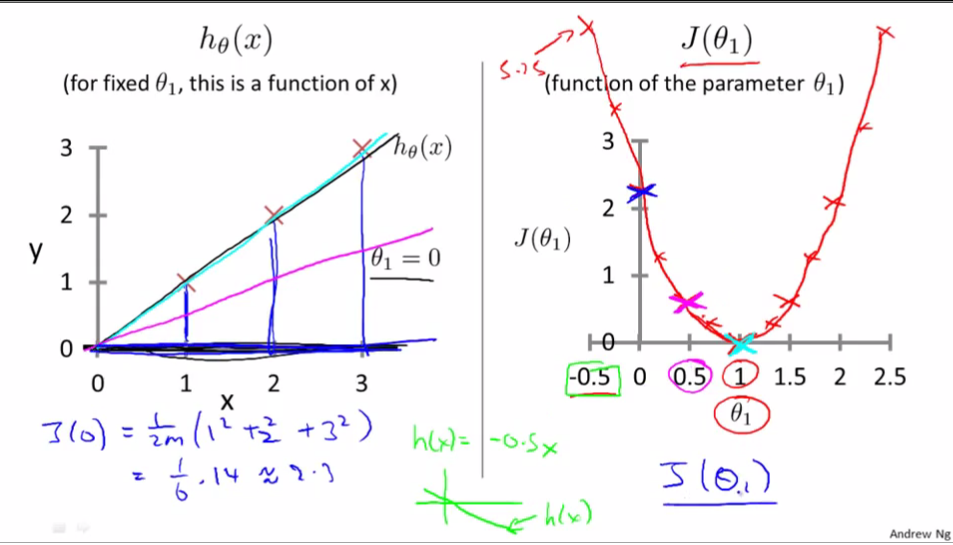
\includegraphics[scale=0.75]{sections/cs229/w1/cost_function.png}
\end{center}
This image shows that for varying parameter values, the cost function changes. In this idealistic example there's a global minimum, the goal of minimized cost, that is very easily followed by a hill-climbing style algorithm.

\subsubsection{Cost Function - Intuition II}
\begin{center}
	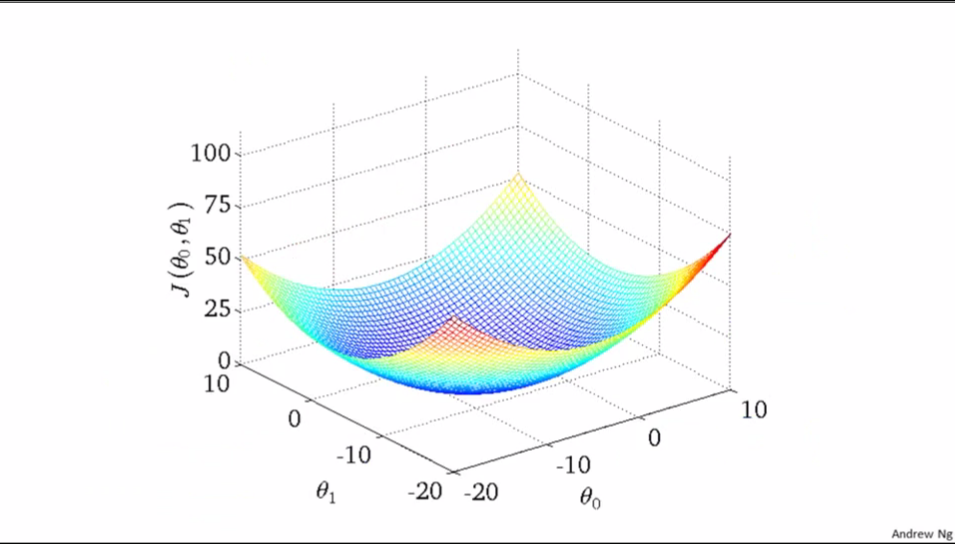
\includegraphics[scale=0.75]{sections/cs229/w1/2d_cost_function.png}
\end{center}
Similarly when you have an additional variable, you want to reach the bottom of this $N$-dimensional hill (note: not all models will have such a perfect hill). 
\begin{itemize}[--]
	\item The gradient gives the direction of maximumal increase on a surface.
	\item We will use a negative gradient to find the `direction' to travel towards the bottom of the hill
	\item Another common way to represent multidimensional cost functions is through contour plots
	\item 
\end{itemize}

	\subsection{Linear Regression with Multiple Variables}
	\subsubsection{Multiple Features}
\begin{itemize}[--]
	\item Instead of just one feature ($x$), we known multiple features ($x_1,\ldots, x_n$). eg. size, number of bedrooms, number of floors, age of home.
	\item $x^{(i)}_j:$ value of feature $j$ in $i^{th}$ training example
	\item Now our hypothesis must account for multiple features: 
		$$h_\theta (x)=\theta_0 + \theta_1 x_1 + \ldots \theta_n x_n$$
	\item Again we define $x_0 = 1$ to simplify future math ($x^{(i)}_0=1$).
	$$x=\begin{bmatrix} x_1\\ \vdots\\ x_n\end{bmatrix}\in \mathbb{R}^{n+1}\text{,  }
		\theta = \begin{bmatrix}\theta_0 \\ \vdots\\ \theta_n\end{bmatrix}\in\mathbb{R}^{n+1}$$
	\item Transposing the $\theta$ vector given our assumption for $x_0^{(i)}$ allows us to simplify our hypothesis into:
		$$h_\theta (x) = \theta^{T}x$$
\end{itemize}

\subsubsection{Gradient Descent for Multiple Variables}
\begin{itemize}[--]
	\item Repeat until convergence ($j=0,\ldots, n$): 
		$$\theta_j := \theta_j \alpha\frac{1}{m}\sum_{i=1}^{m}(h(x^{(i)}-y^{(i)}))x^{(i)}_j$$
	\item This is a valid generalization of the previous formula because of our base case $x^{(i)}_0=1$
\end{itemize}

\subsubsection{Gradient Descent in Practice I - Featuer Scaling}
\begin{itemize}[--]
	\item \textbf{Feature scaling:} if features are on similar scales then we converge more quickly
	\item Your parameters will oscillate along the larger ranged parameter making it's way much slower towards the center (in the case of two variables); whereas, if both axis were equal then you don't have a worst case to fret about
	\begin{center}
		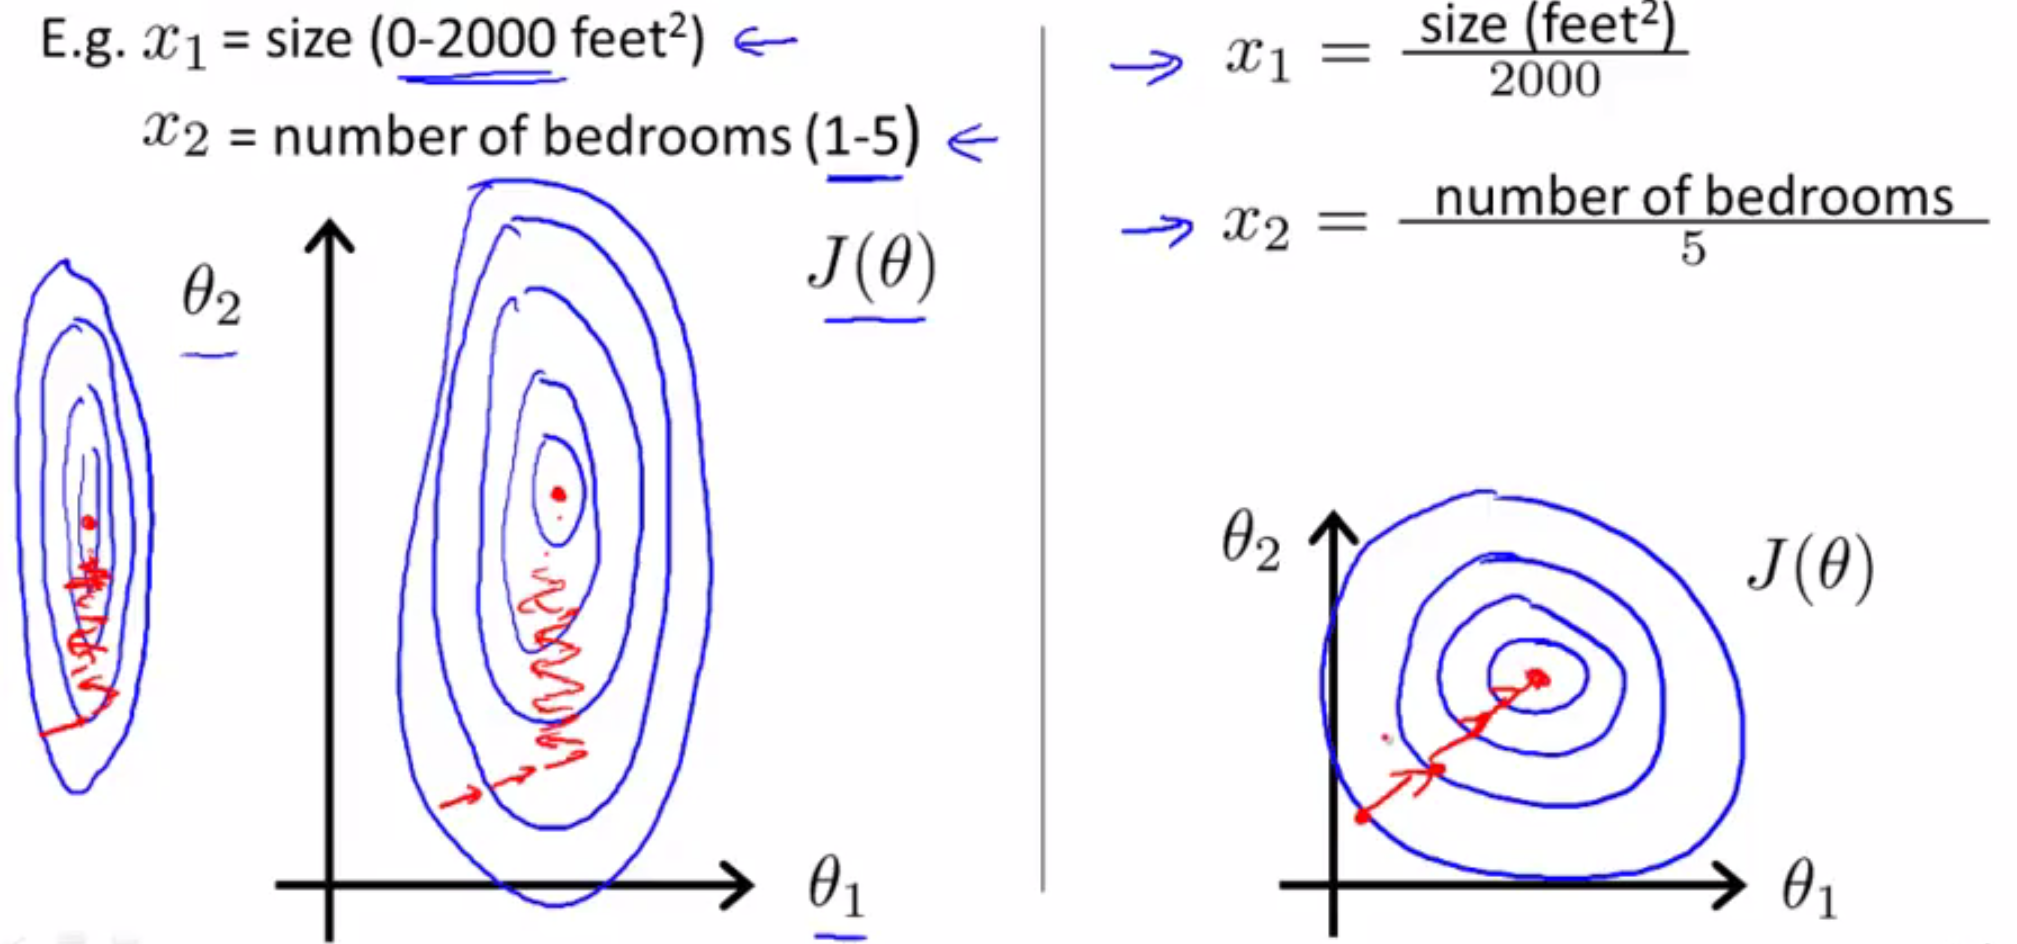
\includegraphics[scale=0.25]{sections/cs229/w2/feature_scaling.png}
	\end{center}

	\item Typically, we want to scale each feature into approximately a $-1\leq x_i \leq 1$ range (same order of magnitude).
	\item \textbf{Mean normalization:} replacing $x_i$ with $x_i-\mu_i$ to make features have approximately zero mean (does not apply to $x_0=1$).
	\item Combining mean normalization and feature scaling we assign $x_i := \frac{x_i-\mu_i}{range_i}$

\end{itemize}

\subsubsection{Gradient Descent in Practice II - Learning Rate}
\begin{itemize}[--]
	\item To ensure gradient descent is working correctly, plot the cost function against the number of iterations. It should converge towards 0, decreasing at every iteration.
	\item The number of iterations required can vary widely for different applications
	\item You can create an automatic convergence test to ensure appropriately ending of gradient descent by checking if the difference between two iterations $\epsilon$ is below a threshold.
	\item If there is any increase in slope, use a smaller $\alpha$
	\item For sufficiently small $\alpha$, $J(\theta )$ should decrease on every iteration
	\item But if $\alpha$ is too small, gradient descent an be slow to converge
	\item To choose $\alpha$ try: $\ldots, 0.001, 0.003, 0.01, 0.03, 0.1, 0.3, 1,\ldots$
\end{itemize}

\subsubsection{Features and Polynomial Regression}
\begin{itemize}[--]
	\item Suppose we have a housing price prediction: $h(x)=\theta_0 + \theta_1 (frontage)+\theta_2 (depth)$
	\item We can define a new feature $(area)=(frontage)(depth)$, that we can use in a new hypothesis $h(x)=\theta_0+\theta_1 (area)$
	\item We can map these hypothesis of more complex features into a linear regression problem: 
	\begin{align*}
		h(x)&=\theta_0 + \theta_1 x_1 + \theta_2 x_2 + \theta_3 x_3    
  		  	&=\theta_0 + \theta_1 (size) + \theta_2 (size)^2 + \theta_3 (size)^3
	\end{align*}

	\item If your features are like those chosen, then feature scaling is very important
	\item There are many more choices for modifications to our features (such as: $\sqrt{}$).
	\item Trying new features can allow you to have a more appropriate model
\end{itemize}

\subsubsection{Normal Equations}
\begin{itemize}[--]
	\item The \textbf{normal equation} allows us to solve for $\theta$ analytically (without iterations)
	\item Intuition: $J(\theta) = a\theta^2+b\theta+c$
	In previous calculus classes you would find the minimum by taking the derivative set equal to 0 and solving for $\theta$. 
	\item This can be extended with partial fractions and solving for every $\theta_j\in\theta$. $$\frac{\partial}{\partial\theta_j}J(\theta)=\ldots=0 \text{    (for every}j\text{)}$$
	\item We construct a matrix from the features and a vector from the solutions as so ($n$ features, $m$ examples):

	\[X=\begin{bmatrix}
		x_0^{(1)} & x_1^{(1)} & \dots & x_n^{(1)} \\
		x_0^{(2)} & x_1^{(2)} & \dots & x_n^{(2)} \\
		\vdots & \vdots & \ddots & \vdots \\
		x_0^{(m)} & x_1^{(m)} & \dots x_n^{(m)} 
	\end{bmatrix} \in \mathbb{R}^{m\times (n+1)}
	 \]

	 \[
	y=\begin{bmatrix}
		y^{(1)} \\
		y^{(2)} \\
		\vdots \\
		y^{(m)}
	\end{bmatrix}\in \mathbb{R}^{m\times 1}
	 \]

	 \item We can then represent the $\theta$ by the \textbf{normal equation} $$\theta = (X^{T}X)^{-1}X^{T}y$$\
	 \item $X$ is entitled the \textbf{design matrix}
	 \item Normal equation does not perform well with a large $n$ due to the computation $(X^{T}X)^{-1}\in\mathbb{n\times n}$ which is typically $\O{n^3}$
\end{itemize}

	\subsection{Logistic Regression}
	\subsubsection{Multiple Features}
\begin{itemize}[--]
	\item 
\end{itemize}


  
	\subsection{Regularization}
	\subsubsection{The Problem of Overfitting}
\begin{itemize}[--]
	\item \textbf{Underfitting}: when a model cannot capture the underlying trend of the data ("high bias")
	\item \textbf{Overfitting}: when a model captures the noise of the data ("high variance")
	\item \textbf{Generalize}: fails to fit to new examples
	\item Overfitting's poor generalization results in low costs not always being correct
	\begin{center}
		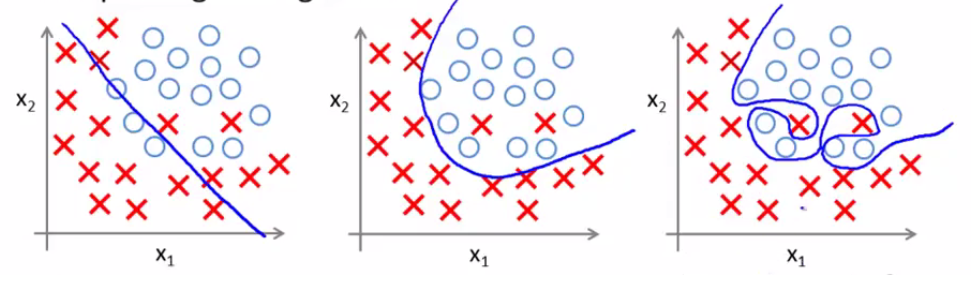
\includegraphics[scale=0.5]{sections/cs229/w4/over-under.png}
	\end{center}

	\item If we have too many features for very little data, overfitting can easily become a big problem.
	\item Options:
	\begin{itemize}
		\item Reduce number of features
		\begin{itemize}
			\item Manually select which features to keep
			\item Model selection algorithm (later in course)
		\end{itemize}
		\item Regularization
		\begin{itemize}
			\item Keep all the features, but reduce magnitude/values of parameters $\theta_j$
			\item Works well when we have a lot of features, each of which contributes a bit to predicting $y$
		\end{itemize}
	\end{itemize}

\end{itemize}

\subsubsection{Cost Function}
\begin{itemize}[--]
	\item Having smaller values for parameters $\theta_0, \theta_1, \ldots, \theta_n$
	\begin{itemize}[--]
		\item ``Simpler'' hypothesis
		\item Less prone to overfitting
	\end{itemize}

	\item To exemplify lets consider the housing scenario:
	\begin{itemize}[--]
		\item Features: $x_1,\ldots, x_100$
		\item Paremeters: $\theta_0, \ldots, \theta_100$
		\item We don't know which ones are complex to shrink, so we modify the cost function to shrink every parameter
		$$J(\theta )=\frac{1}{2m}(\sum_{i=1}^{m}(h(x^{(i)}-y^{(i)})^2 + \lambda\sum_{i=1}^{n}\theta_j^2)$$
		\item We don't penalize $\theta_0$ by convention, because it's a constant and makes very little difference
	\end{itemize}

	\item $\lambda$ is called the regularization parameter. It controls the trade off of fitting the training set well and keeping the parameters small and simple to prevent overfitting
	\item If $\lambda$ is set to be very large we will penalize all the paramters extremely highly resulting which will result in all by the constant being close to zero (fits to a horizontal line). ``Underfit''
\end{itemize}

\subsubsection{Regularized Linear Regression}
\begin{itemize}[--]
	\item Using the new regularized linear regression cost function from the previous section we can now update our gradient descent algorithm to encorporate this modification:
		$$\theta_0 := \theta_0 - \alpha\frac{1}{m}\sum_{i=1}^{m} (h(x^{(i)})-y^{(i)})x_0^{(i)}$$
		$$\theta_j := \theta_j - \alpha ( \frac{1}{m}\sum_{i=1}^{m}(h(x^{(i)})-y{(i)})x)j^{(i)} +\frac{\lambda}{m}\theta_j )$$

	\item The $\theta_j$ $(j=1,\ldots, n)$ term can also be written:
		$$\theta_j := \theta_j (1-\alpha\frac{\lambda}{m}) - \alpha\frac{1}{m}\sum_{i=1}^{m}(h(x^{(i)}) - y^{(i)})x_j^{(i)}$$

	\item The term $(1-\alpha\frac{\lambda}{m})$ is typically $<1$, so this results in shrinking $\theta_j$ by multiplying by a value $<1$, and then performing the same gradient descent function
	\item We also had the normal equation to solve the same problem, and it can also be updated for regularization:
		$$\theta = (X^{T}X+\lambda \left[ \begin{smallmatrix}
			0 & & &\\
			& 1 & &  \\
			& & \ldots & \\
			& & & 1 
		\end{smallmatrix}\right] )X^{T}y$$

	\item Suppose $m\leq n$ then $(X^{T}X)$ will be non-invertible/singular
	\item Regularization will take care of this flaw so long as $\lambda > 0$
\end{itemize}

\subsubsection{Regularized Logistic Regression}
\begin{itemize}[--]
	\item We can also regularize logistic regression in a similar manner
		$$\theta_0 := \theta_0 - \alpha\frac{1}{m}\sum_{i=1}^{m} (h(x^{(i)})-y^{(i)})x_0^{(i)}$$
		$$\theta_j := \theta_j - \alpha ( \frac{1}{m}\sum_{i=1}^{m}(h(x^{(i)})-y{(i)})x)j^{(i)} +\frac{\lambda}{m}\theta_j )$$
		$$h(x)=\frac{1}{1+e^{-\theta^{T}x}}$$
\end{itemize}

	\subsection{Neural Networks: Representation}
	\subsubsection{Non-linear Hypothesis}
\begin{itemize}[--]
	\item Suppose you have a housing classification problem with different features $x_1, \ldots ,x_100$ and if we were to include all quadratic terms for linear classification there would be an enourmous number of terms (~5000 features).
	\item Using linear classifiers has an extremely bad asymptotic complexity (n is typically large)
	\item For example computer vision problems are $\O{n^2}$
	\item Neural networks turn out to be a much better way to solve these style problems
\end{itemize}

\subsubsection{Neurons and the Brain}
\begin{itemize}[--]
	\item Neural networks origins are in algorithms that try to mimic the brain
	\item \textbf{``One learning algorithm hypothesis''}: $x$ cortex can learn whatever is hooked up to it
	\begin{itemize}[--]
		\item Auditory cortex can learn to see
		\item Somatosensory cortex (touch) can learn to see
		\item There is one algorithm that can teach anything to do any function
	\end{itemize}
\end{itemize}

\subsubsection{Model Representation I}
\begin{itemize}[--]
	\item Neural networks work by simulating the neurons in the brain
	\item Has ``input wires'' dendrite
	\item Has ``output wires'' axon
	\item Neuron is a computational unit that takes in inputs and produces an output
	\item Neurons communicate with little spikes of electricity through their axons, which another neuron can receiv with its dendrite
	\item In an artificial neural network we model a neuron as a logistic unit:
	\begin{center}\begin{tikzpicture}[node distance=1cm, auto]
		%Place nodes
		\node (x1) {$x_1$};
		\node [below of=x1] (dots) {$x_2$};
		\node [below of=dots] (xn) {$x_3$};

		\node [cloud, right of=dots] (neuron) {  };

		\node [right of=neuron] (h) {$h_\theta (x)$};

		%Draw edges
		\path [line] (x1) -- (neuron);
		\path [line] (dots) -- (neuron);
		\path [line] (xn) -- (neuron);
		\path [line] (neuron) -- (h);
	\end{tikzpicture}\end{center}

		$$x=\begin{bmatrix} x_0\\ x_1\\ x_2\\ x_3 \end{bmatrix}, \theta=\begin{bmatrix}\theta_0 \\ \theta_1 \\ \theta_2 \\ \theta_3 \end{bmatrix}, h(x)=\frac{1}{1+e^{-\theta^{T}x}}$$

	\begin{itemize}[--]
		\item Here the arrows coming from the $x$ are the input wires
		\item The neuron does the computation
		\item Finally the output comes out
	\end{itemize}

	\item The $x_0$ is called the \textbf{bias unit} and is sometimes omitted because it's constant.
	\item \textbf{Activation function}: defines the output of that node given an input or set of inputs
	\item ``weights'' are synonomous with parameters of the model
	\item Neural networks are groups of neurons strung together

	TODO: Neural Network

	$$a_1^{(2)}=g(\theta_{10}^{(1)}x_0+\theta_{11}^{(1)}x_1+\theta_{12}^{(1)}x_2+\theta_{13}^{(1)}x_3)$$
	$$a_2^{(2)}=g(\theta_{20}^{(1)}x_0+\theta_{21}^{(1)}x_1+\theta_{22}^{(1)}x_2+\theta_{23}^{(1)}x_3)$$
	$$a_3^{(2)}=g(\theta_{30}^{(1)}x_0+\theta_{31}^{(1)}x_1+\theta_{32}^{(1)}x_2+\theta_{33}^{(1)}x_3)$$
	$$h(x)=g(\theta_{10}^{(2)}a_0^{(2)}+\theta_{11}^{(2)}a_1^{(2)}+\theta_{12}^{(2)}a_2^{(2)}+\theta_{13}^{(2)}a_3^{(2)})$$

	\item \textbf{Input layer}: first layer of inputted values
	\item \textbf{Output layer}: the final layer that calculates the output value
	\item \textbf{Hidden layer}: the center layers that don't have known outputs (not input or output layer)
	\item $a_i^{(j)}=$ ``activation'' of unit $i$ in layer $j$
	\item $\theta^{(j)}=$ matrix of weights controlling function mapping from layer $j$ to layer $j+1$
	\item If a network has $s_j$ units in layer $j$, $s_{j+1}$ units in layer $j+1$, then $\theta^{(j)}$ will be of dimension $s_{j+1}\times (s_j + 1)$
\end{itemize}

\subsubsection{Model Representation II}
\begin{itemize}[--]
	\item Consider the previous neural network, where we performed the 4 large equations to calculate the output; we will modify the notation to be of the form:
		$$a_1^{(2)}=g(z_1^{(2)})$$
		$$a_2^{(2)}=g(z_2^{(2)})$$
		$$a_3^{(2)}=g(z_3^{(2)})$$
	\item Let us define:
		$$x=\begin{bmatrix}
			x_0 \\ x_1 \\ x_2 \\ x_3
		\end{bmatrix}, z^{(2)}=\begin{bmatrix}
			z^{(2)}_1 \\ z^{(2)}_2 \\ z^{(2)}_3
		\end{bmatrix}$$
	\item This allows us to perform vectorized calculations:
		$$z^{(2)}=\theta^{(1)}x$$
		$$a^{(2)}=g(z^{(2)})$$
	\item If we instead consider the input layers to be the first layer of activation $a^{(1)}=x$, we may redefine our formulas:
		$$z^{(2)}=\theta^{(1)}a^{(1)}$$
		$$a^{(2)}=g(z^{(2)})$$
	\item We can account for any bias units by including $a_0^{(k)}=1$
		$$h(x)=a^{(3)}=g(z^{(3)})=g(\theta^{(2)}a^{(2)})$$
	\item \textbf{Forward propagation}: information only moves in one direction, forward, from the input nodes, through the hidden nodes (if any) and to the output nodes
	\item If you cover part of the neural network, only showing the last two layers, you'll notice that it's just logistic regression
	\item However instead of using the original features $x_1, \ldots, x_n$, they're using the new features it learned on its own $a_1, \ldots, a_n$
	\item This allows you to use better features than if you were constrained to only your own features, the network has the ability to learn any new features it wants
	\item The \textbf{network architecture} is how the neurons are laid out and connected
\end{itemize}

\subsubsection{Examples and Intuitions I}
\begin{itemize}[--]
	\item Non-linear classification example: XOR/XNOR, is difficult to to model

	TODO Graph

	\item For example we can model simple logical operations with logistic regression:
	\begin{center}
		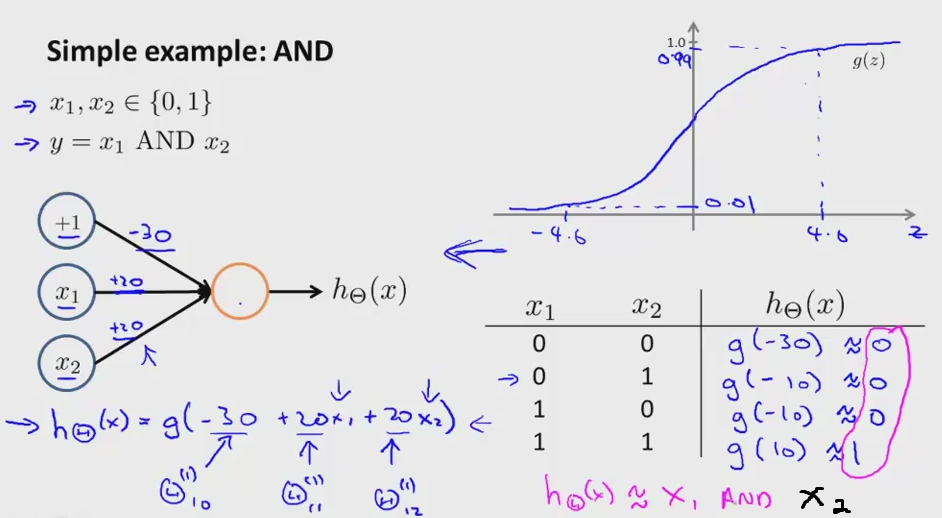
\includegraphics[scale=0.5]{sections/cs229/w5/and_nn.png}
	\end{center}

	\begin{center}
		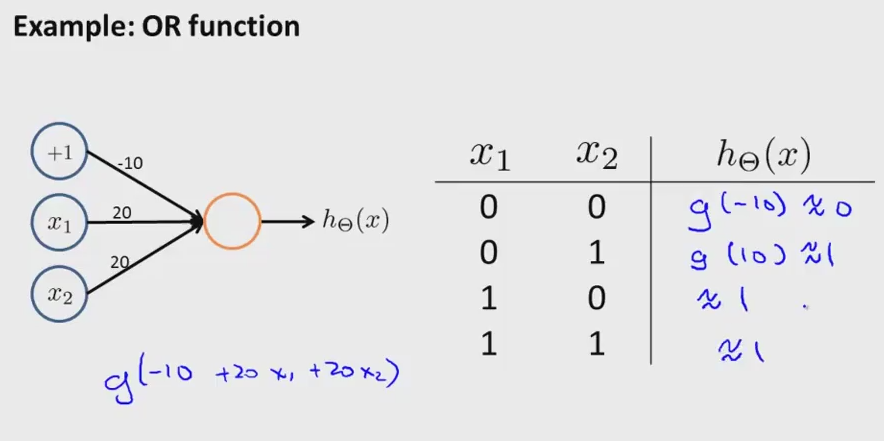
\includegraphics[scale=0.5]{sections/cs229/w5/or_nn.png}
	\end{center}
\end{itemize}

\subsubsection{Examples and Intuitions II}
\begin{itemize}[--]
	\item For models that have non linear boundaries, using a multi-layered network is the best way to approximate the model, for example:
	\begin{center}
		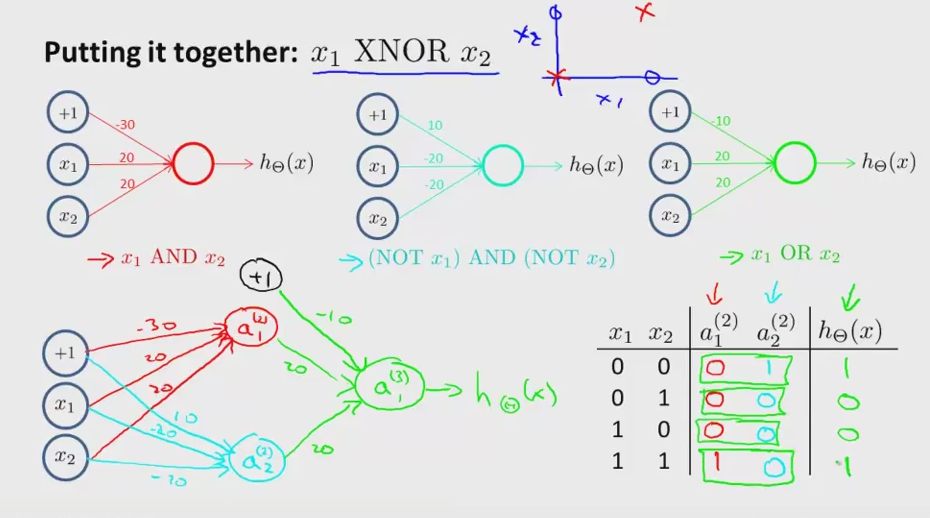
\includegraphics[scale=0.5]{sections/cs229/w5/xnor_nn.png}
	\end{center}

	\item Each layer of the neural network is able to compute even more complex features
	\item The last layer makes the prediction about the correct classification
\end{itemize}

\subsubsection{Multiclass Classification}
\begin{itemize}[--]
	\item Multiclassification is an extension of a one-vs-all 
	\item We want to have the same output units as classes $h(x)\in\mathbb{R}^k$
	\item Each is a classifier for each class, ie. Is it a `1,' is it a `2,' etc..
	\item 
\end{itemize}

	\subsection{Neural Networks: Learning}
	\subsubsection{Cost Function}
\begin{itemize}[--]
	\item Suppose we have:
	\begin{itemize}[--]
		\item Training sets: $\left\{ (x^{(1)}, y^{(1)}),\ldots, (x^{(m)}, y^{(m)})  \right\}$
		\item $m=$ number of training examples
		\item $L=$ total number of layers in network
		\item $s_l=$ number of units (not counting bias unit) in layer $l$
		\item $k=$ number of classes
	\end{itemize}

	\item Binary Classification:
	\begin{itemize}[--]
		\item $y=0\text{ or } 1$
		\item 1 output unit $h(x)\in\mathbb{R}$
		\item $s_l=1$
		\item $k=1$
	\end{itemize}

	\item Multi-class Classification ($K$ classes)
	\begin{itemize}[--]
		\item $y\in\mathbb{R}^K$
		\item $K$ output units
		\item $h(x)\in\mathbb{R}^K$
		\item $s_l=K, (K\geq 3)$
	\end{itemize}

	\item New cost function:
		$$h_{\Theta}(x)\in\mathbb{R}^K, (h_{\Theta}(x))_i=i^{\text{th}}\text{ output}$$
		$$J(\Theta)=-\frac{1}{m}\left[
			\sum_{i=1}^{m}\sum_{k=1}^{K} y_k^{(i)}\log (h(x^{(i)}))_k + (1-y_k^{(i)})\log (1- h(x^{(i)})_k)
			\right] + \frac{\lambda}{2m}\sum_{l=1}^{L-1}\sum_{i=1}^{s_l}\sum_{j=1}^{s_l + 1} (\Theta_{ji}^{(l)})^2$$
\end{itemize}

\subsubsection{Backpropagation Algorithm}
\begin{itemize}[--]
	\item In order to perform gradient descent we need to compute $J(\Theta), \frac{\partial}{\partial\Theta_{ij}}^{(l)} J(\Theta)$
	\item We have already defined $J(\Theta)$, so we just need the partial derivatives.
	\item Intuition: $\delta_j^{(l)}=$ ``error'' of node $j$ in layer $l$
	\item An example is for each output unit (layer $L=4$): $\delta_{j}^{(4)}=a_{j}^{(4)} - y_{j}$
	\item We will comput the $\delta$ for every layer of the neural network
		$$\delta^{(n)} = (\Theta^{(3)})^{T}\delta^{(n+1)} .\times g'(z^{(n)})$$
	\item Where $.\times$ is element-wise multiplication
	\item There is no erro associated with the input layer
	\item The name backpropagation, comes from calculating the error from the back towards the beginning of the network

	\item Suppose we have a training set of $m$ examples
	\item We will set $\Delta_{ij}^{(l)}=0$ (for all $l,i,j$)
	\item This will be used to compute the partial derivatives of the cost function

	TODO: turn into pseudocode

	For $i=1$ to $m$:
		Set $a^{(1)}=x^{(i)}$
		Perform forward propagation to compute $a^{(l)}$ for $l=2,3,\ldots, L$
		Using $y^{(i)}$, comput $\delta^{(L)}=a^{(L)}-y^{(i)}$
		Compute $\delta^{(L-1)}, \delta^{(L-2)}, \ldots, \delta^{(2)}$
		$\Delta_{ij}^{(l)}:=\Delta_{ij}^{(l)} + a_j^{(l)} \delta_i^{(l+1)}$

	\item It's possible to vectorize the final update: $\Delta^{(l)} := \Delta^{(l)} + \delta^{(l+1)} (a^{(l)})^{T}$
	\item After completing the loop we calculate:
		$$D_{ij}^{(l)} := \frac{1}{m}\Delta_{ij}^{(l)} + \lambda\Theta_{ij}^{(l)} \text{ if } j\neq 0$$
		$$D_{ij}^{(l)} := \frac{1}{m}\Delta_{ij}^{(l)} \text{ if } j=0$$
		$$\frac{\partial}{\partial\Theta_{ij}^{(l)}} J(\Theta) = D_{ij}^{(l)}$$
\end{itemize}

\subsubsection{Backpropagation Intuition}
\begin{itemize}[--]
	\item Let us first take another look at forward propagation
	\item We first feed an input into the input layer $x^{(i)}$, then we calculate the second layer $z_1^{(2)}\to a_1^{(2)}$, similarly for the next 2 layers
	\begin{center}
		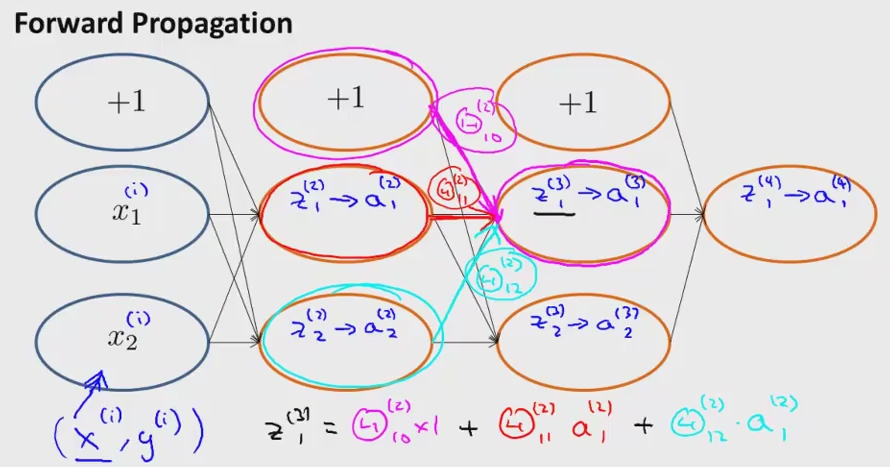
\includegraphics[scale=0.7]{sections/cs229/w6/forward_prop.png}
	\end{center}

	\item If you focus on a single example, the case of 1 output unit, and ignoring regularization ($\lambda = 0$): 
		$$\text{cost}(i)=y^{(i)}\log h(x^{(i)}) + (1-y{(i)} ) \log h(x^{(i)} )$$
	\item Formally, $\delta_j^{(l)}=\frac{\partial}{\partial z_j^{(l)}}\text{cost}(i)\text{ for } j\geq 0$
	\item Backpropagation looks identical, but backwards:
	\begin{center}
		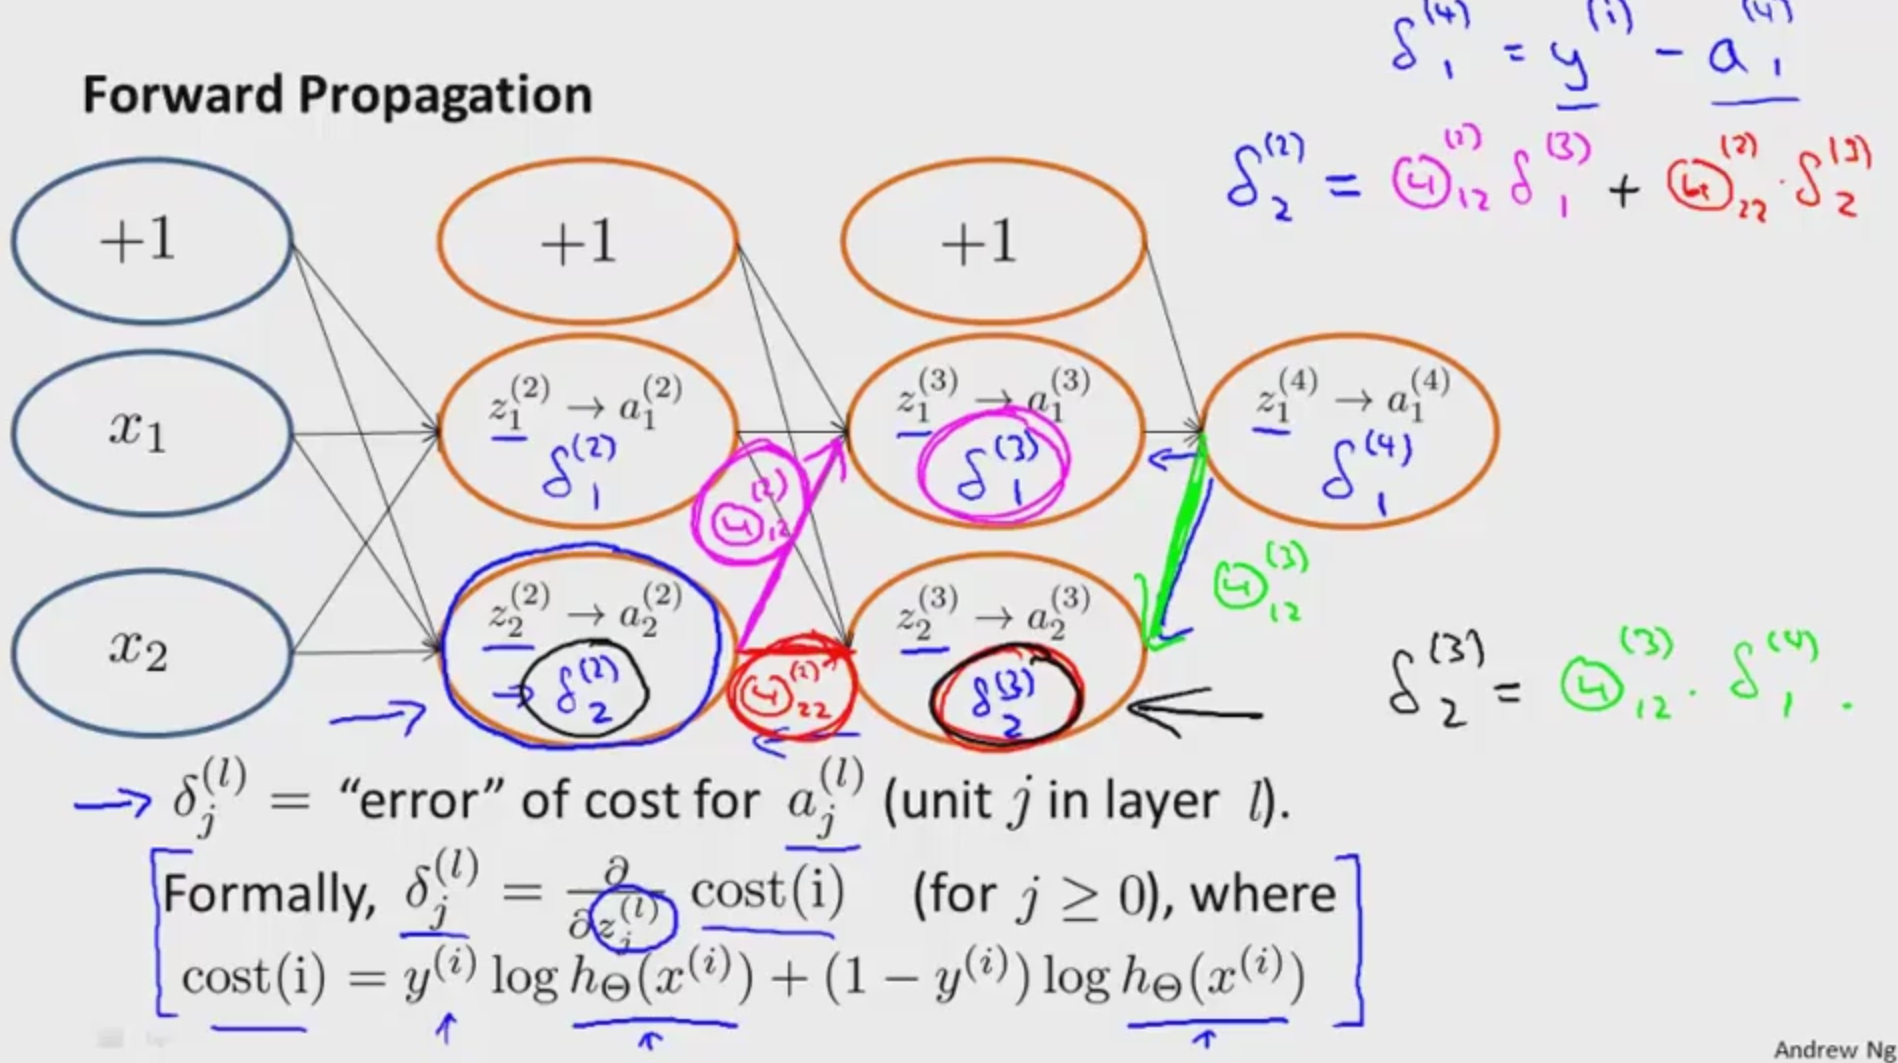
\includegraphics[scale=0.25]{sections/cs229/w6/back_prop.png}
	\end{center}
\end{itemize}

\subsubsection{Implementation Note: Unrolling Parameters}
\begin{itemize}[--]
	\item Our previous use of minfunc and costFunction in octave assumed that $\theta$ and the return would be vectors
	\item You can unroll elements into  large vector:
		thetaVec = [Theta1(:); Theta2(:); Theta3(:)];
	\item You can also change them back into the matrix using reshape:
		Theta1 = reshape(thetaVec(1:size),dim1, dim2);
	\begin{center}
		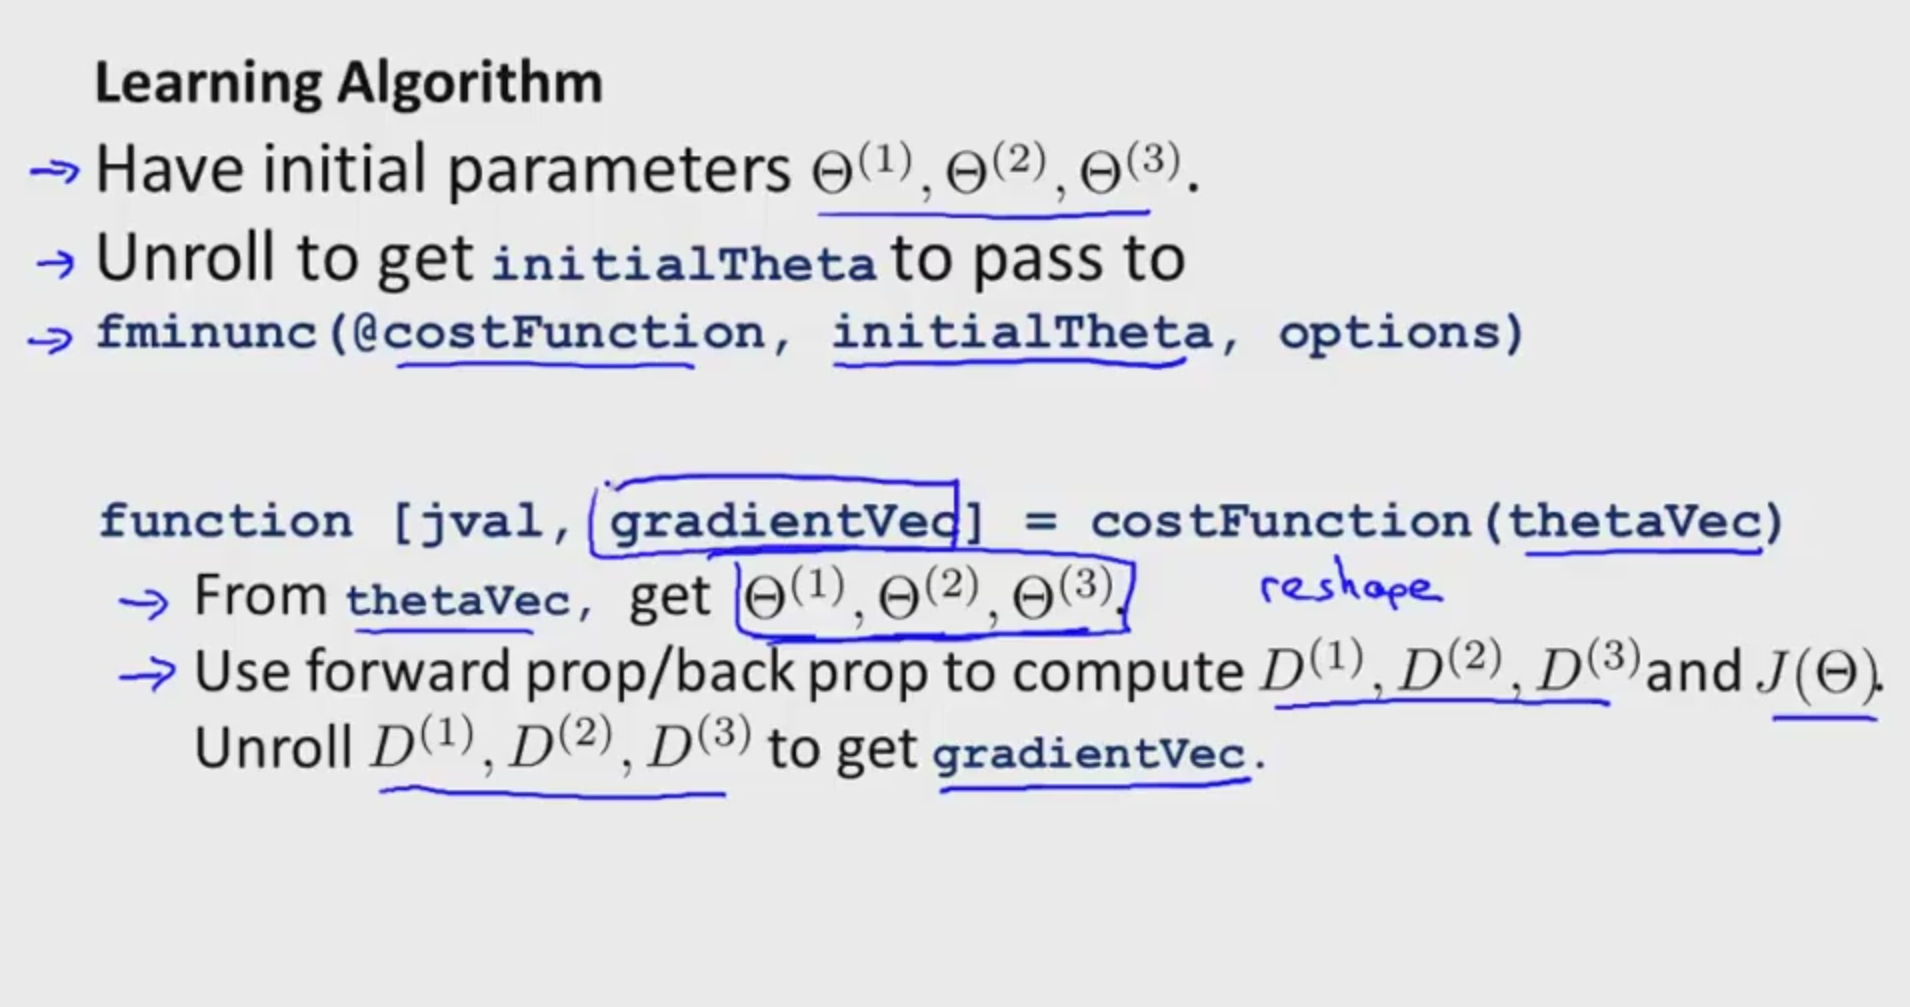
\includegraphics[scale=0.2]{sections/cs229/w6/algo.png}
	\end{center}
\end{itemize}

\subsubsection{Gradient Checking}
\begin{itemize}[--]
	\item Suppose you have a function $J(\Theta)$, and we want to estimate the derivative at $\theta\in\mathbb{R}$.
	\item We consider the points $\theta - \epsilon$ and $\theta + \epsilon$, and draw a line through these points and use the slope of this line as an approximation
	\item This gives our approximation as:
		$$\frac{d}{d\Theta} J(\Theta) = \frac{J(\Theta + \epsilon) - J(\Theta - \epsilon)}{2\epsilon}$$
	\item A good value for epsilon is: $\epsilon= 10^{-4}$
	\item Now consider $\theta\in\mathbb{R}^{n}$
	\item We can calculate the derivative for each element the same as we did for the single variable. Holding the other variables constant
	\item We then can compare this approximate derivative to the backpropagation to check that they're approximately the same
	\item Don't do gradient checking once you start learning, because it will be very slow
	\item j
\end{itemize}

\subsubsection{Random Initialization}
\begin{itemize}[--]
	\item Initializing all the parameters in a neural network, does not work like it did in our previous algorithms
	\item After each update, parameters corresponding to inputs going into each of two hidden units are identical
	\item This results in not being able to develop more complex features
	\item Instead, we will now initialize each $\Theta_{ij}^{(l)}$ to a random value in $\left[ -\epsilon, \epsilon \right]$
	\item The goal is ``symmetry breaking''
\end{itemize}

\subsubsection{Putting it Together}
\begin{itemize}[--]
	\item We must pick a network architecture (connectivity pattern between neurons)
	\item Reasonable default: 1 hidden layer, or if >1 hidden layer, have same number of hidden units in every layer (usually the more the better)
	\item Training a neural network:
	\begin{itemize}[--]
		\item Randomly initialize weights
		\item Implement forward propagation to get $h_{\Theta} (x^{(i)})$ for any $x^{(i)}$
		\item Impelement code to cmpute cost function $J(\Theta)$
		\item Implement backprop to compute partial derivatives $\frac{\partial}{\partial \Theta_{jk}^{(l)}} J(\Theta)$
		\item Perform forward propagation and backpropagation using each example
		\item Use gradient checking to compare partial derivatives computed using backpropagation vs. using numerical estimate of gradient of $J$. Then disable gradient checking code.
		\item Use gradient descent or advanced optimization method with backpropagation to try and minimize $J$ as a function of parameters $\Theta$
	\end{itemize}

	\item $J(\Theta )$ is non-convex, and can get stuck in local optimum
	
\end{itemize}

	\subsection{Advice for Applying Machine Learning}
	\subsubsection{Deciding What to Try Next}
\begin{itemize}[--]
	\item Suppose ou've trained your model, but it is largely error prone. What should you try next?
	\begin{itemize}[--]
		\item Get more training examples
		\item Try smaller sets of features
		\item Try getting additional features
		\item Try adding polynomial features
		\item Try decreasing $\lambda$
		\item Try increasing $\lambda$
	\end{itemize}

	\item \textbf{Diagnostic}: A test that you can run to gain insight what is/isn't working with a learning algorithm, and gain guidance as to how best to improve its performance
	\item Diagnostics can take time to implement, but oding so can be a very good use of your time
\end{itemize}

\subsubsection{Evaluating a Hypothesis}
\begin{itemize}[--]
	\item \textbf{Overfitting}: fails to generalize to new example not in training set
	\item How do we determine if it overfits?
	\item Suppose we have data set ${(x^{(i)}, y^{(i)} )}$, we will split the data into two sets: \textbf{training set}, and \textbf{test set}
	\item We will typically assign $~70\%$ to be the training set, and the remainder $~30\%$ to be the test set
	\item $m_{test}=$ number of test example
	\item Training/testing procedure for linear regression:
	\begin{itemize}[--]
		\item Learn parameter $\theta$ from training data (minimizing training error J($\theta$))
		\item Compute test set error:
			$$J_{test}(\theta_{training})=\frac{1}{2m_{test}}\sum_{i=1}^{m){test}}(h(x_{test}^{(i)}) - y_{test}^{(i)})^2$$
	\end{itemize} 

	\item Training/testing procedure for logistic regression:
	\begin{itemize}[--]
		\item Learn parameter $\theta$g from trainin data 
		\item Compute test set error:
			$$J_{test}(\theta_{training})=\frac{-1}{m_{test}}\sum_{i=1}^{m){test}}y_{test}^{(i)}\log h(x_{test}^{(i)}) + (1-y_{test}^{(i)}) \log h(x_{test}^{(i)} )$$
		\item Misclassification error (0/1 misclassification error):
			$$\text{err}(h(x), y)=\begin{cases}
				1 &\text{if } h(x)\geq 0.5 (y=0), \text{ or if } h(x)<0.5 (y=1)\\
				0 &\text{otherwise}
			\end{cases}$$
			$$\text{Test error} = \frac{1}{m_{test}}\sum_{i=1}^{m_{test}}\text{err}(h(x_{test}^{(i)}, y^{(i)})$$
	\end{itemize} 


\end{itemize}

\subsubsection{Model Selection and Train/Validation/Test Sets}
\begin{itemize}[--]
	\item If you consider adding another parameter to your model that is: $d=$degree of polynomial
		$$h(x;d)=\sum_{i=0}^{d}\theta_i x^{i}$$
	\item If we denote the parameters for each respctive model as $\theta^{(d)}$, we can then consider $J_{test}(\theta^{(d)}$ for each hypothesis
	\item Suppose we choose a model $\theta^{(5)}$, the problem with this system is it is likely to be an optimistic estimate of generalization error; namely, we fit the new parameter $d$ to the test set
	\item It is no longer fair to reuse the test set on this model to test it, because it's already favoring it
	\item Now we will split up the dataset into 3 pieces: \textbf{training set}, \textbf{cross validation set (cv)}, \textbf{test set}
	\item A typical split is 60\%-20\%-20\%, favoring the training set
	\item $m_{cv}=$ number of cross validation examples
	\item Training error:
		$$J_{train}(\theta) = \frac{1}{2m}\sum_{i=1}^{m} (h(x^{(i)}) - y^{(i)})^2$$
	\item Cross Validation error
		$$J_{cv}(\theta) = \frac{1}{2m_{cv}}\sum_{i=1}^{m_{cv}} (h(x^{(i)}_{cv}) - y^{(i)}_{cv})^2$$
	\item Test error
		$$J_{test}(\theta) = \frac{1}{2m_{test}}\sum_{i=1}^{m_{test}} (h(x^{(i)}_{test}) - y^{(i)}_{test})^2$$
	\item Now instead of the test set, we will use the cross validation set to select the model
	\item We will select the model based on the minimum of $J_{cv}(\theta^{(d)})$
	\item j

\end{itemize}


\subsubsection{Diagnosing Bias vs. Variance}
\begin{itemize}[--]
	\item Underfitting/overfitting problems
	\item Overfit = high variance
	\item Underfit = high bias
	\begin{center}
		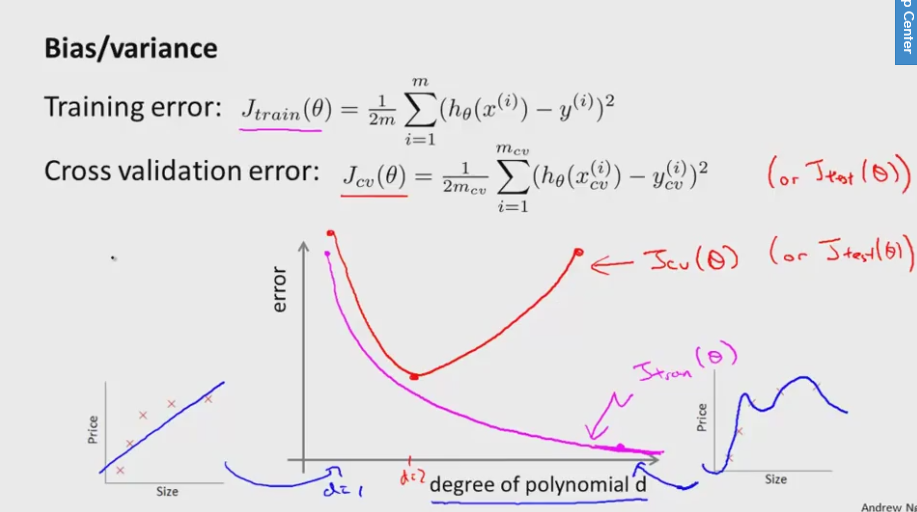
\includegraphics[scale=0.5]{sections/cs229/w7/bias_var.png}
	\end{center}

	\item High bias is shown on the left, where you have a low order polynomial with a large error
	\item High variance is shown on the right, where you have a high decree polynomial with a large error
	\item Your model suffers from high bias (underfit) problem if the training error is high and the cv is approximately the same.
	\item Your model suffers from high variance (overfit) if the training is low (fit well) while the cv error is much greater than the training error
\end{itemize}


\subsubsection{Regularization and Bias/Variance}
\begin{itemize}
	\item In regularization we have a regularization term with a variable $\lambda$
	\begin{center}
		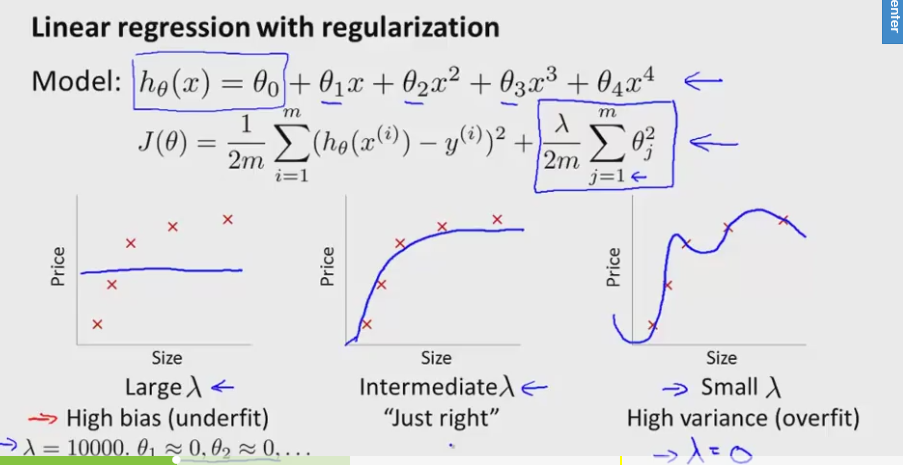
\includegraphics[scale=0.5]{sections/cs229/w7/reg.png}
	\end{center}

	\item When you have a large $\lambda$ all parameters are heavily penalized, so only the constant term remains
	\item Contrasting, when we have a small $\lambda$ we maintain our very high variance overfitting
	\item We want to find the ``just right'' value
	\item Choosing the regularization parameter $\lambda$
	\begin{itemize}
		\item Try multiples of $\lambda=0,0.01,0.02,0.04,0.08,\ldots, 10$
		\item Let the models of each value of $\lambda$ be $\theta^{(n)}$
		\item Choose the smallest $J_{cv}(\theta{(n)})$
	\end{itemize}

	\begin{center}
		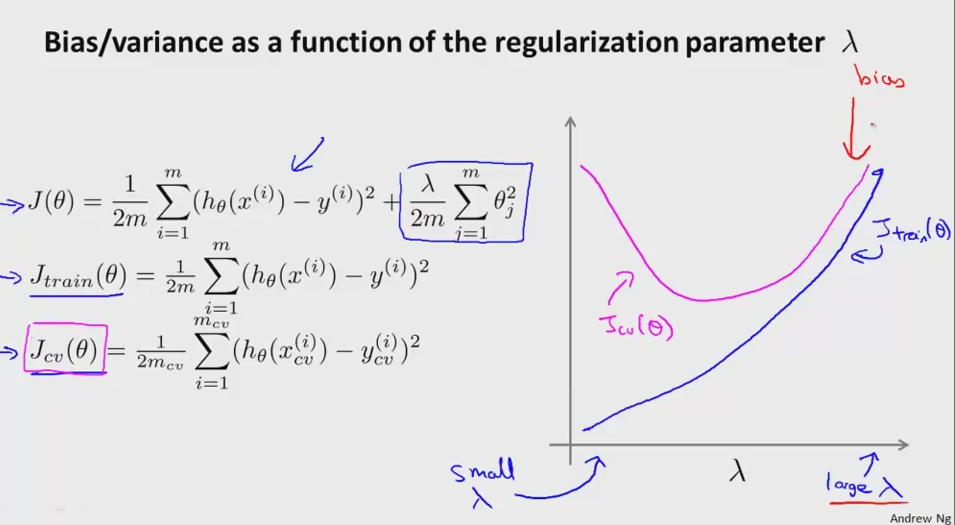
\includegraphics[scale=0.5]{sections/cs229/w7/lambda.png}
	\end{center}
	\item For small $\lambda$ you have little penalty and are able to fit your data well 
	\item The cross validation error is very high when $\lambda$ is small because you fit the too perfectly to other data set
\end{itemize}

\subsubsection{Learning Curves}
\begin{itemize}[--]
	\item Plot $J_{train}$ or $J_{cv}$ against $m$ (training set size)
	\item To do this we will deliberatly limit our training set size to complete the graph at lower points

	\item Suppose you have a high bais, If we were to increase the training set size you end up with a similar straight line
	\item The cv error will plateau out because the line can't conform any better to the data 
	\item The training set also has a similar error because it's unable to also conform to the data
	\item It has a high bias because both errors are high
	\item If a learning algorithm is suffering from high bias, getting more training data will not (by itself) help much.
	\begin{center}
		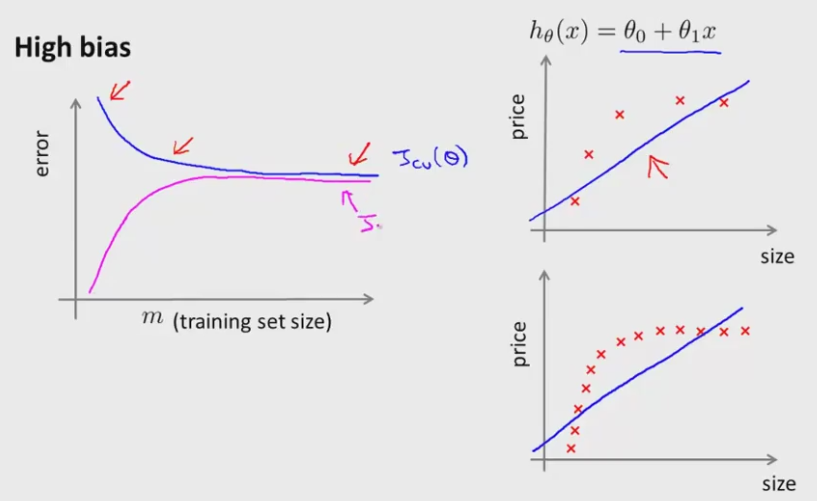
\includegraphics[scale=0.5]{sections/cs229/w7/bias.png}
	\end{center}

	\item Suppose now you have high variance, we will fit the data very well; however, it will largely overfit the data
	\item Since we can very easily fit the data our training error will remain low
	\item However, the cross validation error will remain high because it's too perfectly fitted for other data points
	\item The variance occurs do to this large gap in error between cv and training
	\item If a learning algorithm is suffering from high variance, getting more training data is likely to help.
	\begin{center}
		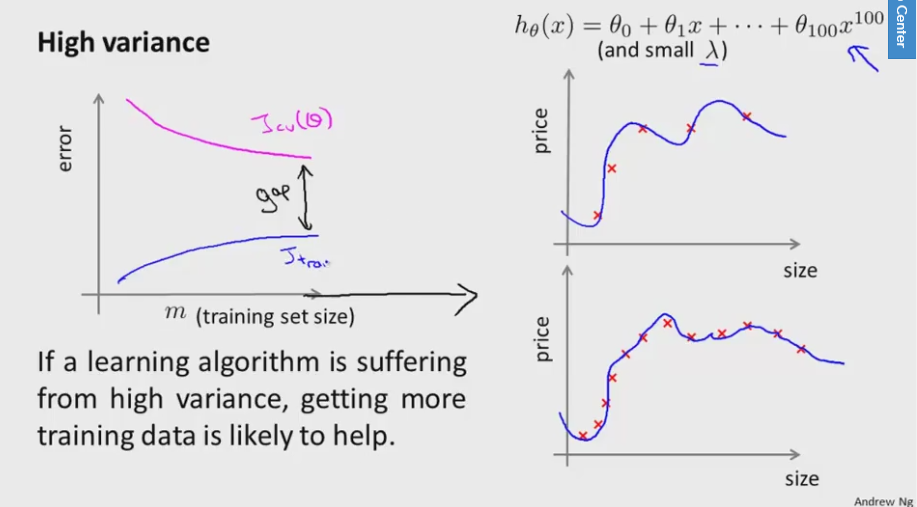
\includegraphics[scale=0.5]{sections/cs229/w7/var.png}
	\end{center}


\end{itemize} 

\subsubsection{Deciding What to Do Next Revisited}
\begin{itemize}[--]
	\item What should you try next?
	\begin{itemize}[--]
		\item Get more training examples $\to$ fixes high variance
		\item Try smaller sets of features  $\to$ fixes high variance
		\item Try getting additional features $\to$ fixes high bias (typically)
		\item Try adding polynomial features $\to$ fixes hih bias
		\item Try decreasing $\lambda$ $\to$ fixes high bias (less penalty for complex features)
		\item Try increasing $\lambda$ $\to$ fixes high variance (more penalty for complex features)
	\end{itemize}

	\item ``Small'' neural networks: fewer parameters; more prone to underfitting; computationally cheaper

	TODO: Draw

	\item ``Large'' neural network: more parameters; more prone to overfitting; computationally more expensive; use regularization to address overfitting

	TODO: Draw

	\item Try using the training/cv/test sets to determine the best choice for number of hidden layers
\end{itemize}


	\subsection{Machine Learning System Design}
	\subsubsection{Prioritizing What to Work On}
\begin{itemize}[--]
	\item Building a spam Classifier:
	\begin{itemize}[--]
		\item Supervised learning problem.
		\item $x=$features of email
		\item $y=$ spam (1) or not spam (0)
		\item Featurs $x$: choose 100 words indicative of spam/not spam
		\item $\vec{x}=$ 1 when the corresponding word appears, and 0 otherwise (eg. andrew is the first word, and it's in the email $x\left[ 0\right]=1$)
		\item Note: in practice, take most frequently occuring $n$ words (10000 to 50000) in training set, rather than manually pick 100 words
	\end{itemize}

	\item How to spend our time to make it have low error?
	\begin{itemize}[--]
		\item Collect lots of data
		\begin{itemize}[--]
			\item eg. ``honeypot'' project
		\end{itemize}

		\item Develop sophisticated features, for example based on email routing information (from email header)
		\item Develop sophisticated features for message body, eg. should ``discount'' and ``discounts'' be treated as the same word? How about ``deal'' and ``Dealer''? Features about punctuation?
		\item Develop sophisticated algorithm to detect misspellings (eg. m0rtgages, med1cine, w4tches)
	\end{itemize}
\end{itemize}

\subsubsection{Error Analysis}
\begin{itemize}[--]
	\item Recommended approach:
	\begin{itemize}
		\item Start with a simple algorithm that you can implement quickly. Implement it and test it on our cross-validation data
		\item Plot learning curves to decide if more data, more features, etc. are likely to help.
		\item Error analysis: Manually examine the examples (in cross validation set) that your algorithm made errors on. See if you spot any systematic trend in what type of examples it is making errors on
	\end{itemize}

	\item This allows evidence to decide our decisions, and not gut feelings
	\item Manually categorize errors when doing analysis:
	\begin{itemize}[--]
		\item What type of error is it
		\item What cues (features) you think would have helped the algorithm classify them correctly
	\end{itemize}

	\item The importance of numerical evaluation:
	\item Should discount/discounts/discounted/discounting be treated as the same word?
	\item Can use ``stemming'' software (eg. Porter stemmer)
	\item 
\end{itemize}

\subsubsection{Error Metrics for Skewed Classes}
\begin{itemize}[--]
	\item j
\end{itemize}

\subsubsection{Trading Off Precision and Recall}
\begin{itemize}[--]
	\item j
\end{itemize}

\subsubsection{Data For Machine Learning}
\begin{itemize}[--]
	\item j
\end{itemize}


	\subsection{Support Vector Machines}
	\subsubsection{Optimization Objective}
\begin{itemize}[--]
	\item In logistic regression we had the sigmoid activation function, and the hypthosis: $h(x)=\frac{1}{1+e^{-\theta^T x}}$
	\item If we have an example where $y=1$, we want $h(x)=1$, this implies $\theta^{T}x \gg 0$
	\item Conversly, if $y=0$, we want $h(x)=0\to \theta^{T}x\ll 0$
	\item When $y=1$ only the first term of the cost function wil matter ($-y\log\frac{1}{1+e^{-\theta^T x}}$)
	\item If we plot this as a function of $z=\theta^T x$ we get the  following curve
	\begin{center}
		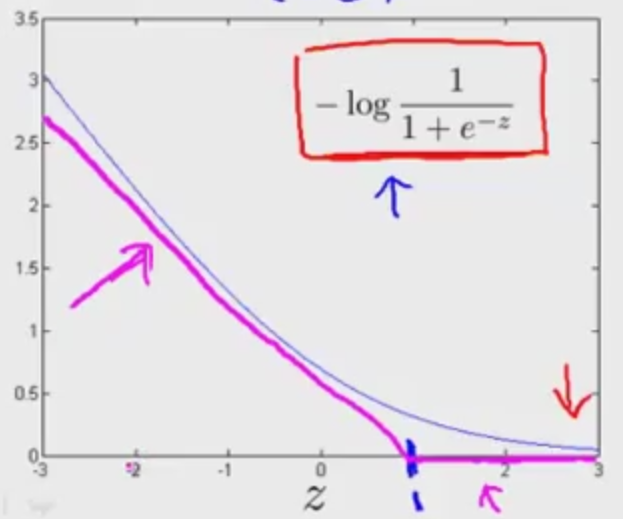
\includegraphics[scale=0.5]{sections/cs229/w9/y_1.png}
	\end{center}
	\item The purple line will be our SVM's cost when $y=1$, which is made up of two line segments

	\item Similarly for when $y=0$ (second term of cost function) we have the same following graphs:
	\begin{center}
		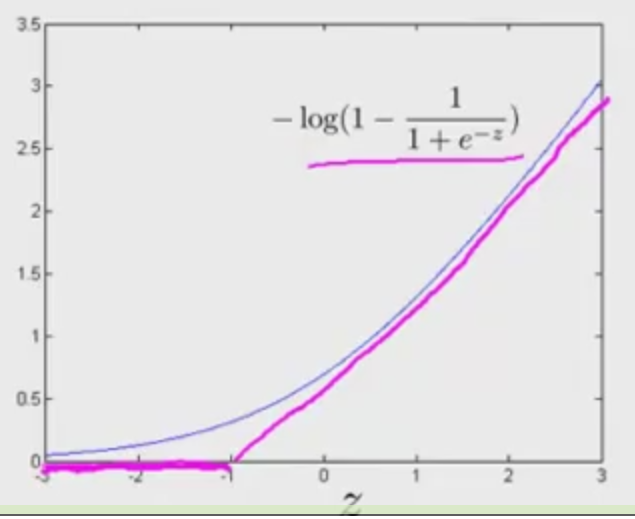
\includegraphics[scale=0.5]{sections/cs229/w9/y_2.png}
	\end{center}

	\item We will denote the SVM's cost when $y=0$ to be $\text{cost}_1 (z)$, similarly when $y=0$, $\text{cost}_0 (z)$
	\item Logistic regression's cost function:
		$$\min_{\theta}\frac{1}{m} \left[ \sum_{i=1}^{m} y^{(i)} (-\log{h(x^{(i)})}) + (1-y^{(i)})((-\log{1-h(x^{(i)})}))\right] + \frac{\lambda}{2m}\sum_{j=1}^{n}\theta_{j}^{2}$$
	\item Support vector machine's cost function:
		$$\min_{\theta}\frac{1}{m} \left[ \sum_{i=1}^{m} y^{(i)} \text{cost}_1(\theta^{T}x^{(i)}) + (1-y^{(i)})\text{cost}_0 (\theta^{T}x^{(i)})\right] + \frac{\lambda}{2m}\sum_{j=1}^{n}\theta_{j}^{2}$$
	\item We should be able to remove the constant, since the minimization problem will take care of reducing it:
		$$\min_{\theta} \left[ \sum_{i=1}^{m} y^{(i)} \text{cost}_1(\theta^{T}x^{(i)}) + (1-y^{(i)})\text{cost}_0 (\theta^{T}x^{(i)})\right] + \frac{\lambda}{2}\sum_{j=1}^{n}\theta_{j}^{2}$$
	\item Also, for SVM we will use a different parameter to control the weight of the penalty term: $A+\lambda B\to CA+B$, where $C$ is our new term
	\item Having learned the parameters $\theta$, this is the hypothesis for the SVM:
		$$
			h(x)=\begin{cases}
				1 & \text{if } \theta^{T}x\geq 0 \\
				0 & \text{otherwise}
			\end{cases}
		$$
\end{itemize}

\subsubsection{Large Margin Intuition}
\begin{itemize}[--]
	\item -
	\begin{center}
		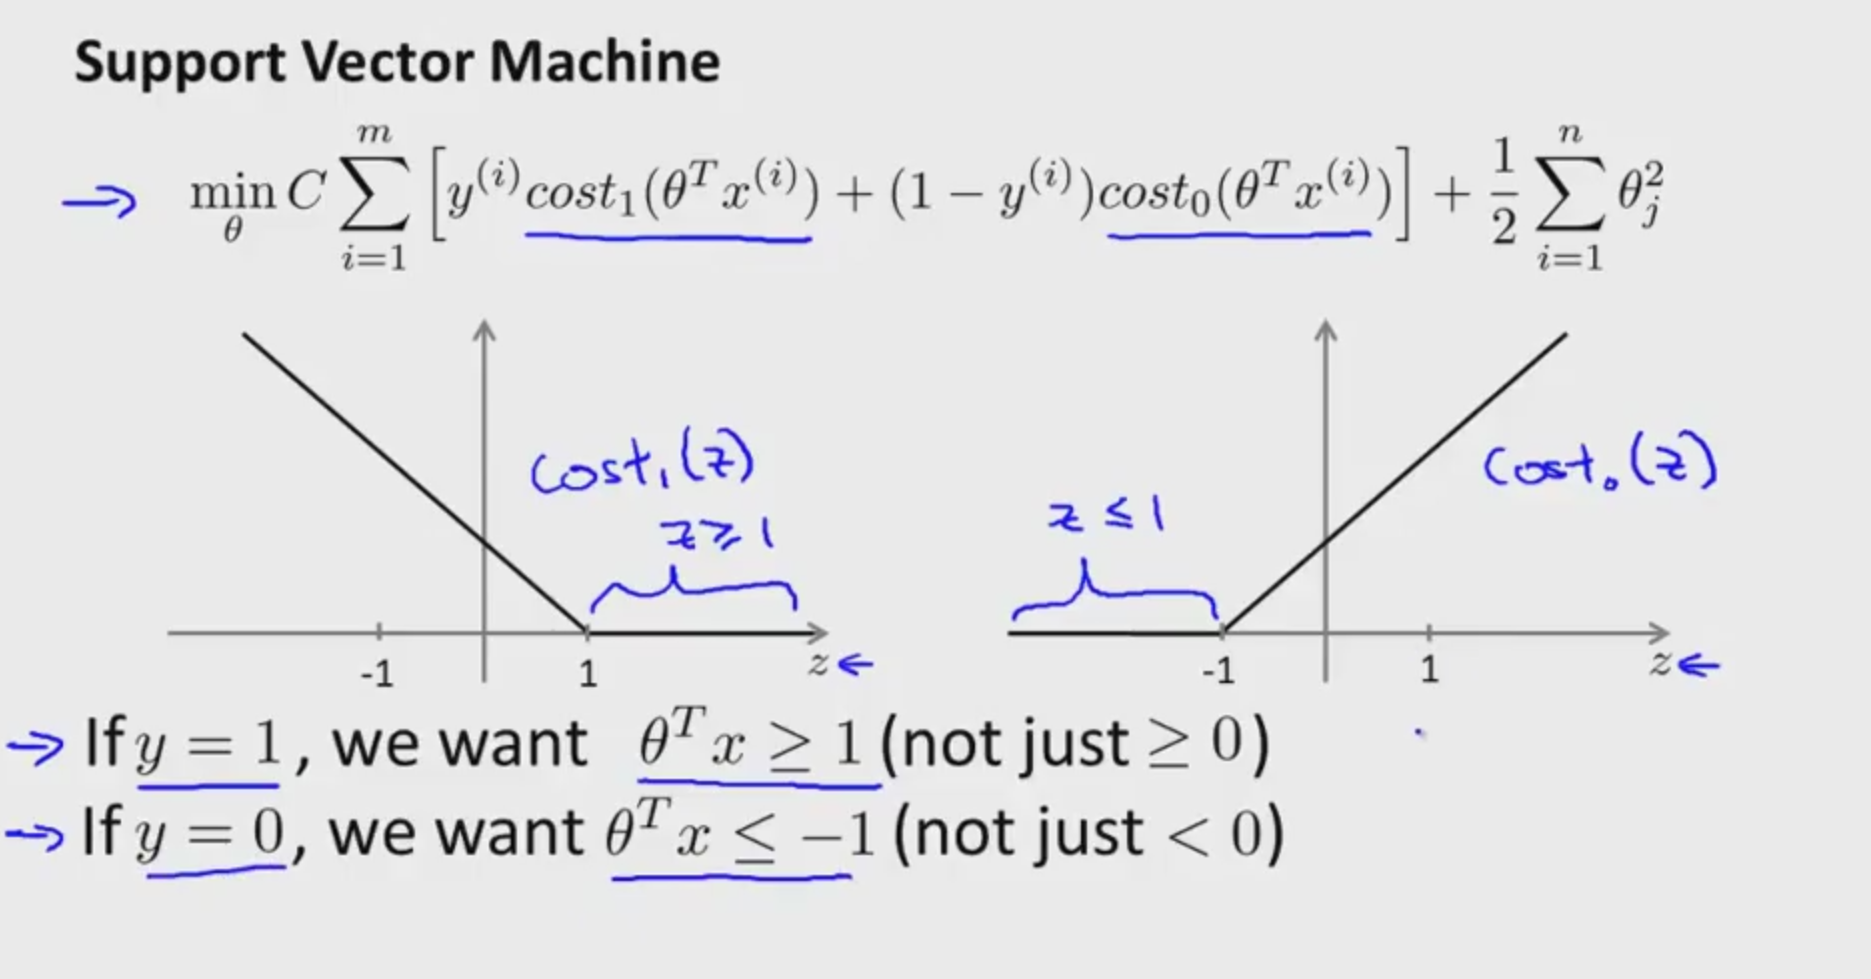
\includegraphics[scale=0.5]{sections/cs229/w9/svm.png}
	\end{center}

	\item To make these cost functions small, we want:
	\begin{align*}
		\theta^{T}x\geq 1 &\text{If } y=1 \\
		\theta^{T}x\leq -1 &\text{If} y=0
	\end{align*}

	\item However, if you just barely get the example right (0 instead of +/- 1), where you stlil have some cost
	\item This builds an extra safety margin factor, still predicting the correct result but there's another ``level'' where you will have no cost
	\item If $C$ is very large, and we want our first cost term to be 0, so our resulting cost function is:
		$$\min_{\theta}\frac{1}{2}\sum_{i=1}^{n}\theta_{j}^{2}$$
	\item This is subject to the constraint: 
	\begin{align*}
		\theta^{T}x^{(i)}\geq 1  & \text{if } y^{(i)}=1\\
		\theta^{T}x^{(i)}\leq -1 & \text{if } y^{(i)}=0
	\end{align*}

	\item When you solve this optimization problem, you get a linearly separable example sets (can be divided by lines into their classes).
	\begin{center}
		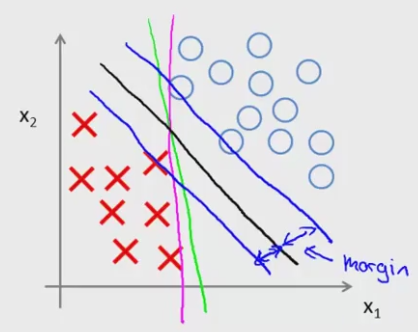
\includegraphics[scale=0.5]{sections/cs229/w9/margin.png}
	\end{center}

	\item There exists many different lines (green/purple) that can fit this division; however, the svm will find the black (most natural looking) dividing line
	\item This line has the largest margin from the classes (the blue lines)
	\item The distance from the predicted line and the nearest item is the margin
	\item The svm is called a \textbf{large margin classifier} because it finds the largest margin for its model
	\item Consider adding an outlier as shown below, that the large margin would not be the `best' idea. If $C$ was very large, this is how the svm will handle the outlier. However, it wasn't, you'd still have hte black decision boundar
	\begin{center}
		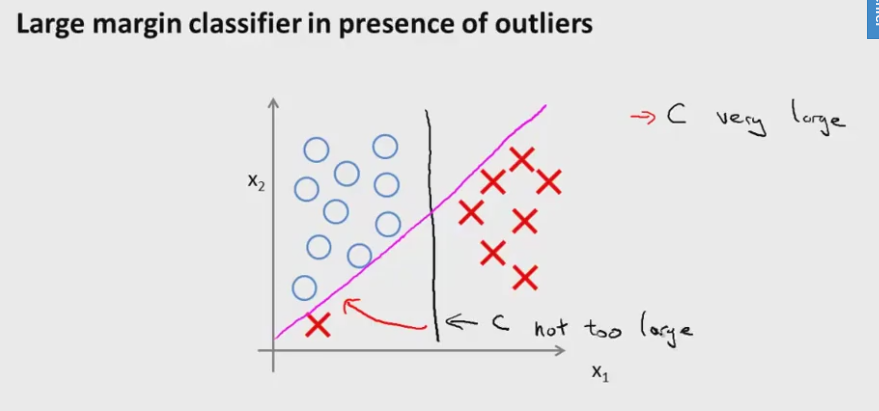
\includegraphics[scale=0.5]{sections/cs229/w9/outlier.png}
	\end{center}
\end{itemize}

\subsubsection{Mathematics Behind Large Margin Classification}
\begin{itemize}[--]
	\item In the case of 2 features, where $\theta_0=0$
		$$\min_{\theta}\frac{1}{2}\sum_{j=1}^{n}\theta_j^2=\frac{1}{2}||\theta||^2$$

		\begin{center}
			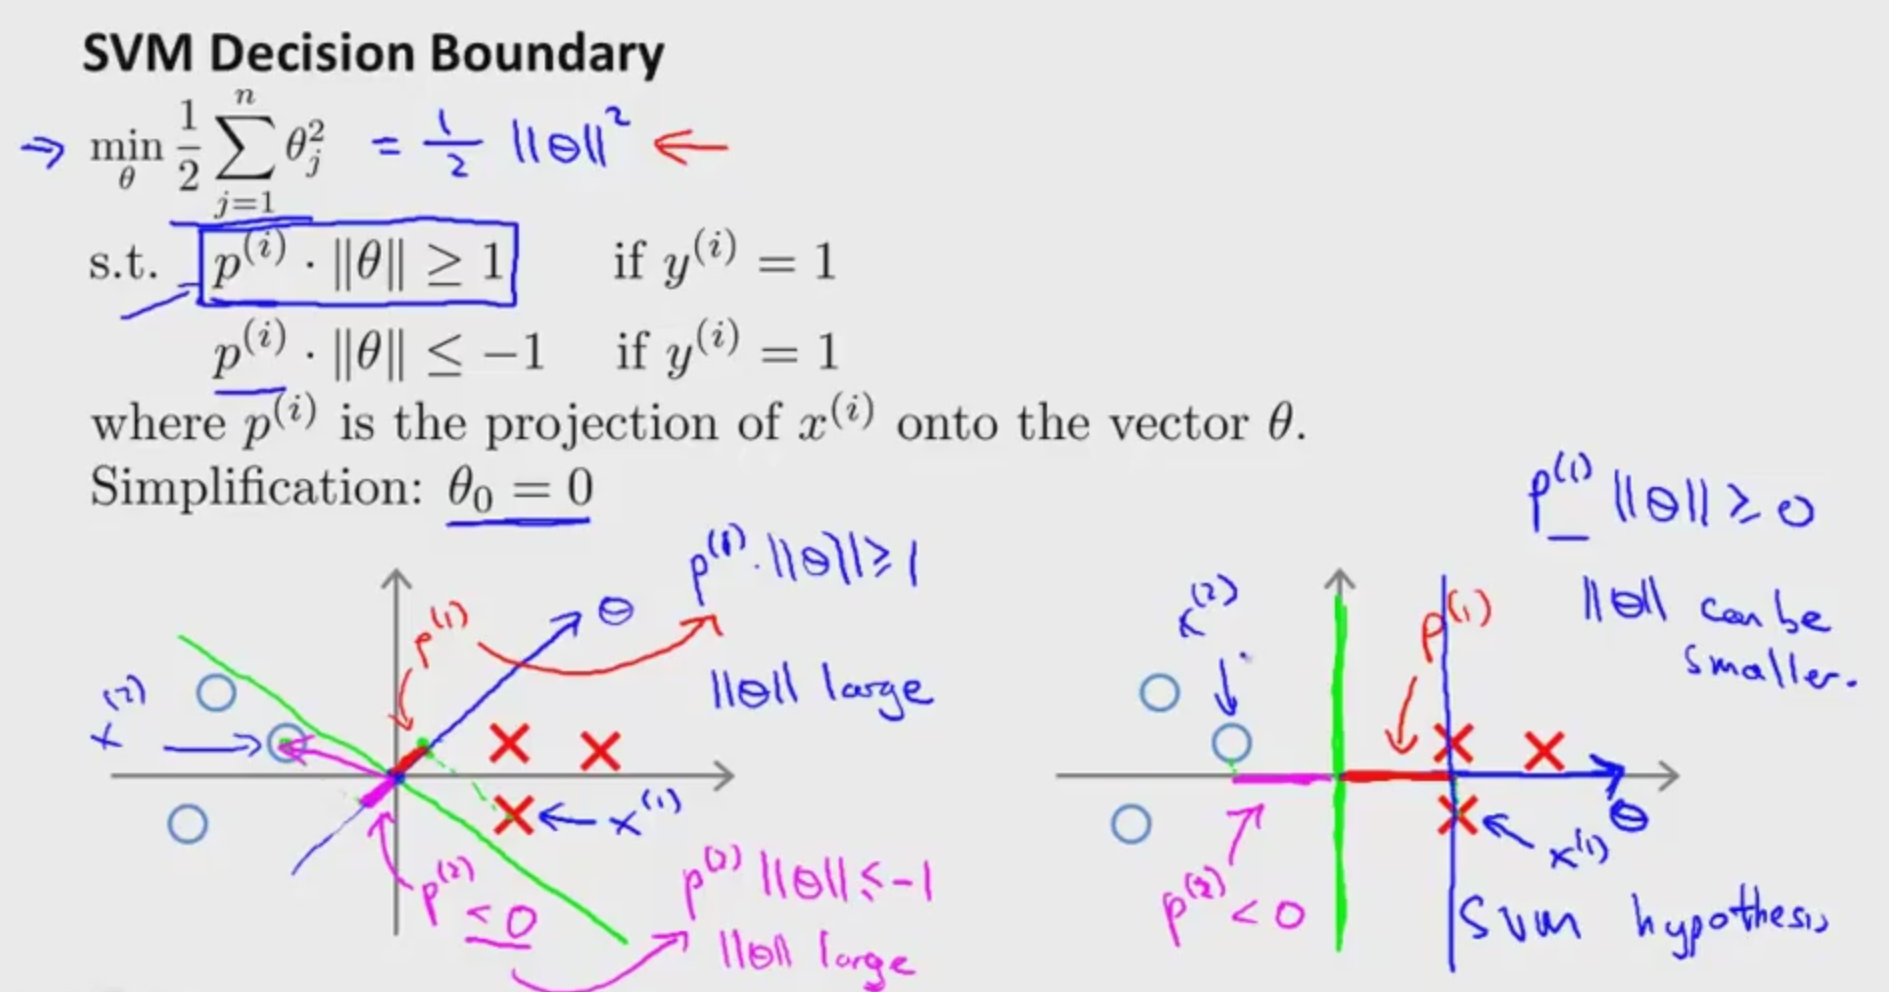
\includegraphics[scale=0.25]{sections/cs229/w9/boundary.png}
		\end{center}

	\item The margin works by trying to get the projectionss of the $y=1$ examples to be large positive values ($\theta$ points towards them, so they have large projections)
	\item This also results in very large negative values for the $y=0$
	\item The $\theta_0 = 0$ assumption, allows this simplification where decision boundary fits to the origin (the ideas proven here work $\theta\neq 0$ as well)
\end{itemize}

\subsubsection{Kernels I}
\begin{itemize}[--]
	\item One way to find a complex non-linear decision boundary is complex polynomials
	\item Another way to denote this is:
		$$\theta_0 + \theta_1 f_1 + \theta_2 f_2 + \ldots$$
	\item In this case:
		$$f_1=x_1, f_2=x_2, f_3=x_1 x_2, f_4=x_1^2, \ldots$$
	\item Is there a different/better chocie of the features $f_1, f_2,\ldots$?
	\item Given $x$, compute new feature depending on proximity to landmarks $l^{(1)}, l^{(2)}, l^{(2)}$
	\item One possible feature: $f_1=\text{similarity}(x,l^{(1)}=\text{exp}(-frac{||x-l^{(2)}||^2}{2\sigma^2})$
	\item For this example, we will also define our second \& third feature similarly: $f_n=\text{similarity}(x,l^{(n)})$
	\item This similarity function is called the \textbf{gaussian kernels}
	\item The idea of the similarity function is called the \textbf{kernel}
	\item If $x\approx l^{(1)}$, then $f_1=\approx \text{exp}(-\frac{0^2}{2\sigma})\approx 1$
	\item If $x$ is far from $l^{(1)}$ then $f_1\approx 0$
	\item So these measure how close $x$ is to the landmarks
	\item You can consider a guassian curve on the 3rd dimension, where the closer you get to the landmark, the higher up the hill (the corresponding value of the feature)
	\item As you increase $\sigma^2$ the value falls away much slower (higher variance tolerated)
	\item Example:
	\begin{center}
		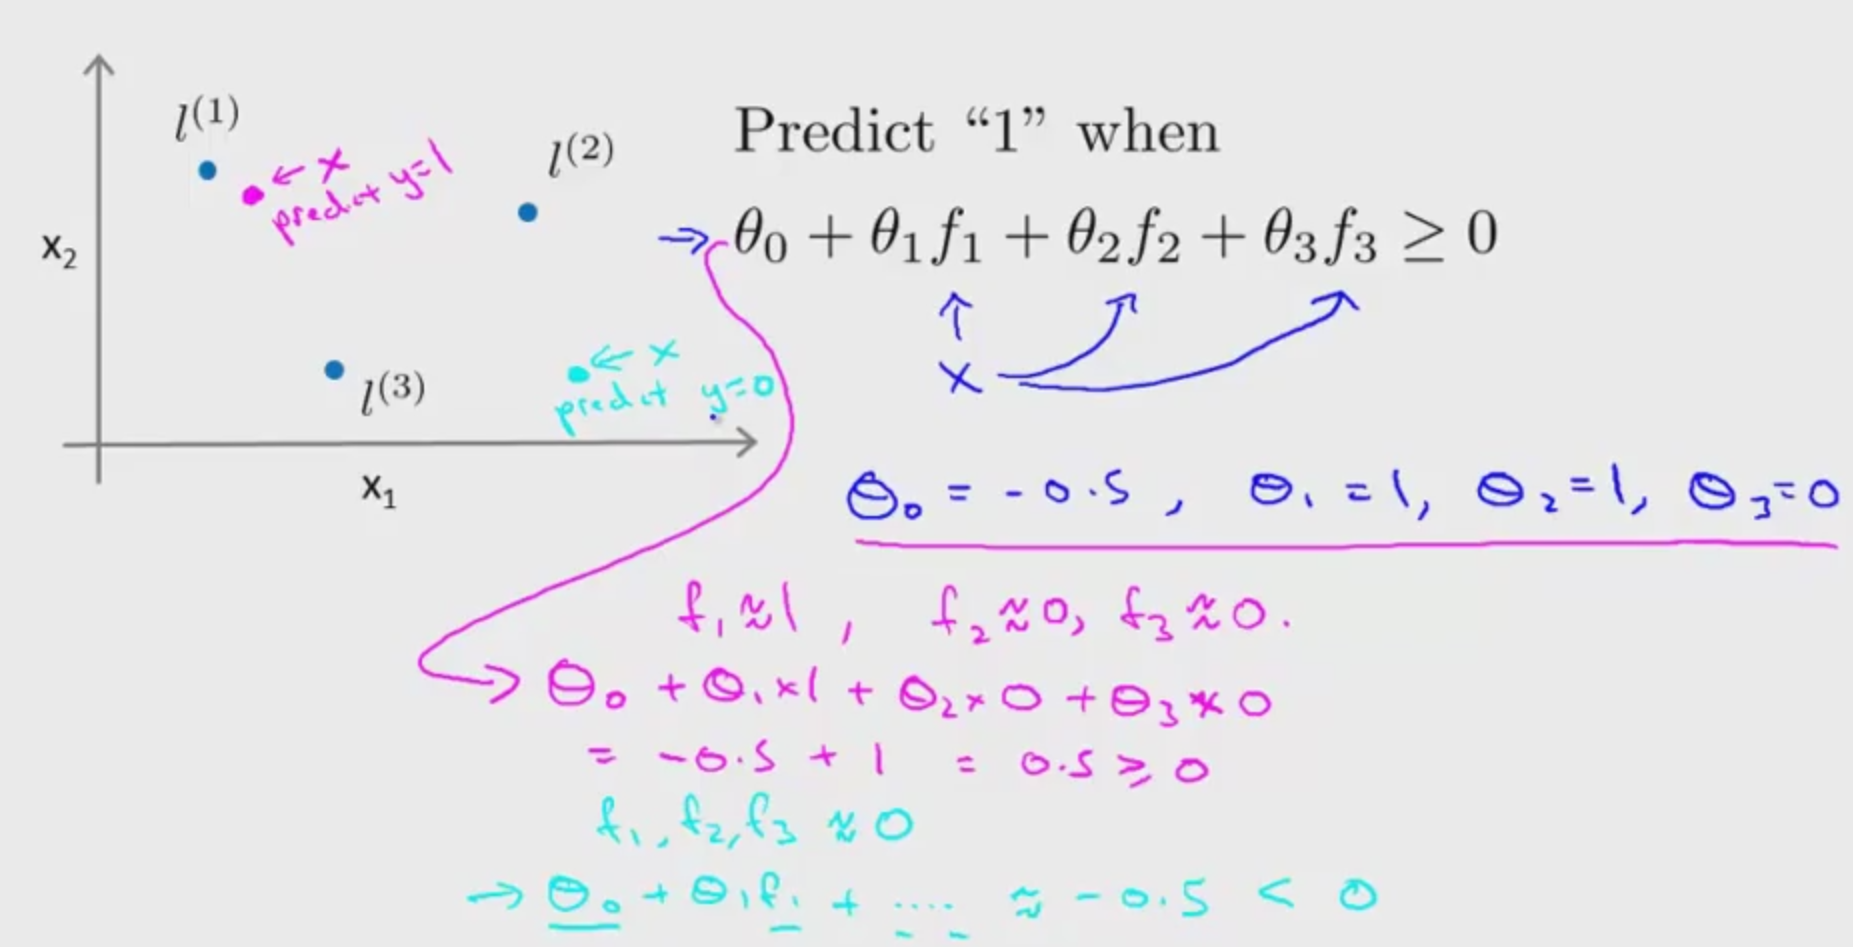
\includegraphics[scale=0.25]{sections/cs229/w9/ex_lm.png}
	\end{center}
\end{itemize}

\subsubsection{Kernels II}
\begin{itemize}[--]
	\item Where do we get $l^{(1)}, l^{(2)}, \ldots$?
	\item Given $m$ training examples, we choose $l^{(1)}, \ldots, l^{(m)}=x^{(m)}$
	\item And our features: $f_m=\text{similarity}(x, l^{(m)}$
	\item We can now represent our training example $i$ as a stacked vector all of all of the new features: 
		$$f^{(i)}=\begin{bmatrix}
			f_0^{(i)}\\
			\vdots \\
			f_m^{(i)}
		\end{bmatrix}$$

	\item SVM with Kernels
	\begin{itemize}[--]
		\item Hypothesis: Given $x$, compute features $f\in\mathbb{R}^{m+1}$
		\item Predict $y=1$ if $\theta^{T}f\geq 0$
		\item Training, by solving:
			$$\min_{\theta} C\sum_{i=1}^{m}y^{(i)}cost_i (\theta^{T}f^{(i)}) + (1-y{(i)})cost_0 (\theta^{T}f^{(i)}) + \frac{1}{2}\sum_{j=1}^{m}\theta_j^2$$
		\item Note: we are ignoring $\theta_0$ in our second term
	\end{itemize}

	\item SVM parameters:
	\begin{itemize}[--]
		\item One of the choices you need to make is what value of $C$ you would like to use
		\item Large $C$: lower bias, high variance
		\item Small $C$: higher bias, low variance
		\item We also need to choice $\sigma^2$
		\item Large $\sigma^2$: featurs $f_i$ vary more smoothly (varies slowly). Higher bias, lower variance.
		\item Small $\sigma^2$: features $f_i$ vary less smoothly (sharper change). Lower bias, higher variance
		\item 
	\end{itemize}
\end{itemize}

\subsubsection{Using an SVM}
\begin{itemize}[--]
	\item When using software packages to computer svm you need to specify:
	\begin{itemize}[--]
		\item Choice of parameter $C$
		\item Choice of kernel (similarity function)
		\item Choice of parameter $\sigma^2$
	\end{itemize}

	\item \textbf{Linear Kernel}: gives standard linear classifier
	\item Why might you choose a gaussian kernel? If $x\in\mathbb{R}^n$, n small andor large. Then the gaussian kernel can help with this very complex models
	\item If it asks you to provide a function to compute the kernel function, \textbf{perform feature scaling before using the kernel}
	\item Only kernels that satsify the condition ``Mercer's Theorem'' to make sure SVM packages' optimizations run correctly, and do not diverge
	\item Many off-the-shelf kernels available:
	\begin{itemize}[--]
		\item Polynomial kernel: $k(x,l;c,p)=(x^T l+c)^p,$
		\item More esoteric: string kernel, chi-square kernel, histogram intersection kernel, $\ldots$
	\end{itemize}

	\item Use the cross-validation set to decide on a kernel

	\item Many svm packages already ahve built-in multi-in multi-class classification unctionality. Otherwie, use one-vs-all method.

	\item Logistic regression vs. svm
	\begin{itemize}[--]
		\item If the number of training examples ($m$) is greater than the number of features ($n$), the typical approach is logistic regression over svm 
		\item If $n$ is small, and $m$ is intermediate ($n=1-1000,m=10-10000$) use svm with guassian kernel
		\item If $n$ is small and $m$ is large, create/add more features, then use logistic regression or svm without a kernel
		\item Neural network likely to work well for most of these settings, but may be slower to train
	\end{itemize}

	\item SVM is convex, so you will always find the global optimum
\end{itemize}

	\subsection{Clustering}
	\subsubsection{Unsupervised Learning: Introduction}
\begin{itemize}[--]
	\item In supervised learning we're given a training set $\{(x^{(m)}, y^{(m)})\}$, we try and find the decision boundary
	\item In \textbf{unsupervised learning} we're given a training set $\{x^{(m)}\}$, give it to an algorithm and try and find structure
	\item An example is a clustering algorithm, which finds data that close together
	\item Applications of clusterin: market segmentation, social network analysis, organize computing clusters, astronomical data analysis
\end{itemize}

\subsubsection{K-Means Algorithm}
\begin{itemize}[--]
	\item Randomly initialize two points, called the \textbf{cluster centroids}
	\begin{center}
		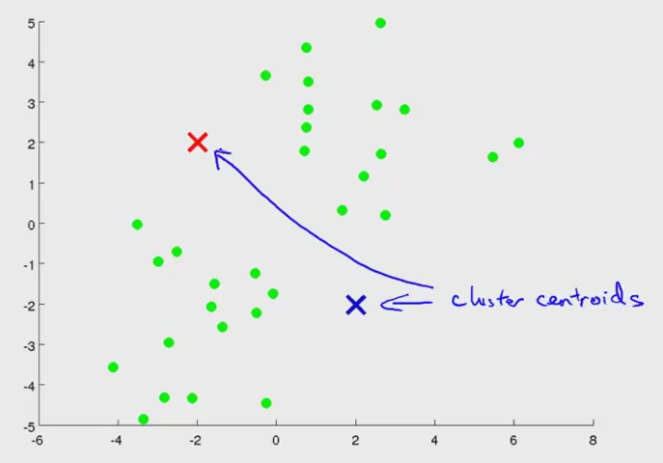
\includegraphics[scale=0.5]{sections/cs229/w10/kmeans1.png}
	\end{center}

	\item You should have a cluster centroid for each group you want 
	\item There's two steps: cluster assignment, and move centroid
	\item \textbf{Cluster assignment}: go through each example, and depending on which cluster it is closer to it will assign it to one of the centroids
	\begin{center}
		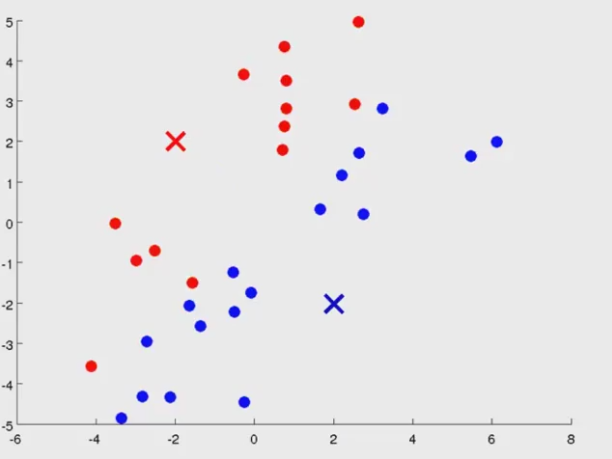
\includegraphics[scale=0.5]{sections/cs229/w10/kmeans2.png}
	\end{center}
	\item \textbf{Move centroid}: move the centroids to the mean of all the same groupped points
	\begin{center}
		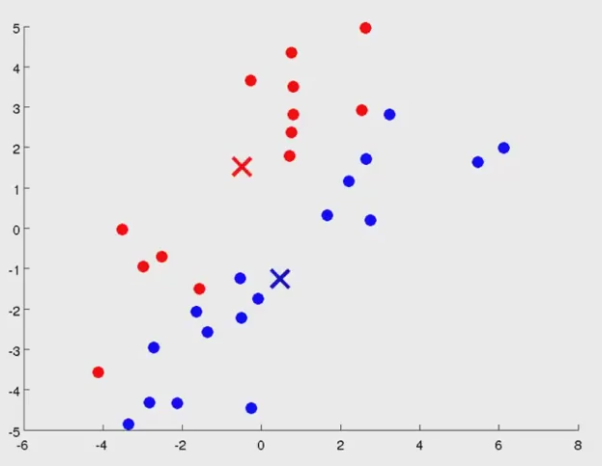
\includegraphics[scale=0.5]{sections/cs229/w10/kmeans3.png}
	\end{center}

	\item Then you repeat this process until the movement of the centroids
	\begin{center}
		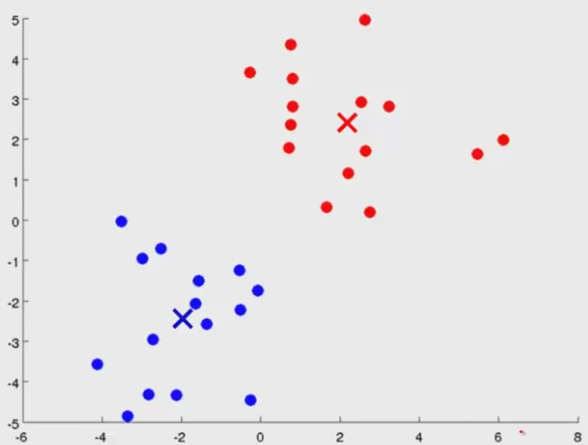
\includegraphics[scale=0.5]{sections/cs229/w10/kmeans4.png}
	\end{center}

	\item \textbf{$K$-means Algorithm}
	\begin{itemize}[--]
		\item Input:
		\begin{itemize}[--]
			\item $K$ (number of clusters)
			\item Training set $\{ x^{(1)}, \ldots, x^{(m)}\}$
		\end{itemize}
		\item $x^{(i)}\in\mathbb{R}^n $ (drop $x_0=1$ convention)
		\item Randomly initialize $K$ cluster centroids $\mu_1,\ldots, \mu_k \in\mathbb{R}^n$
		\item Repeat: TODO: pseudo-code markup
		\begin{itemize}[--]
			\item for $i=1$ to $m$
			\begin{itemize}[--]
				\item $c^{(i)} :=$ index (from 1 to $K$) of cluster centroid closest to $x^{(i)}$ ($\min_k ||x^{(i)} -\mu_k||^2$)
			\end{itemize}
			\item for $k=1$ to $K$
			\begin{itemize}[--]
				\item $\mu_k :=$ average (mean) of points assigned to cluster $k$
			\end{itemize}
		\end{itemize}
	\end{itemize}
\end{itemize}

\subsubsection{Optimization Objective}
\begin{itemize}[--]
	\item $\mu_c (i):=$ cluster centroid of cluster to which example $x^{(i)}$ has been asigned ($x^{(i)}\to 5$, $c^{(i)}=5$, $\mu_{c^{(i)}} =\mu_5$)
	\item Optimzation Objective:
		$$J(c^{(1)},\ldots, c^{(m)}, \mu_1,\ldots, \mu_K )=\frac{1}{m}\sum_{i=1}^{m}||x^{(i)}-\mu_{c^{(i)}}||^2$$
		$$\min_{c^{(1)},\ldots, c^{(m)}, \mu_1, \ldots, \mu_K} J(\ldots )$$
	\item The cluster assignment step, can be shown to be this minimization process of the cost function to the group assignment holding the centroids constant
	\item The moving centroids minimize with respect to the centroids
\end{itemize}

\subsubsection{Random Initialization}
\begin{itemize}[--]
	\item Instead of random centroids, randomly pick $K$ training examples, and set $\mu_1,\ldots, \mu_k$ be these $K$ examples
	\item There exists local optimum, to prevent this we may run the entire $K$-means algorithm, and choose the lowest cost solution
	\item If $K=2-10$, doing local random initializations to find optimal, works well; however, if $K$ is larger then this tends to fall apart
\end{itemize}

\subsubsection{Choosing the Number of Clusters}
\begin{itemize}[--]
	\item The most common way is to manually choose it based on observations.
	\item There exists situations, where it's ambiguous the true number of clusters:
	\begin{center}
		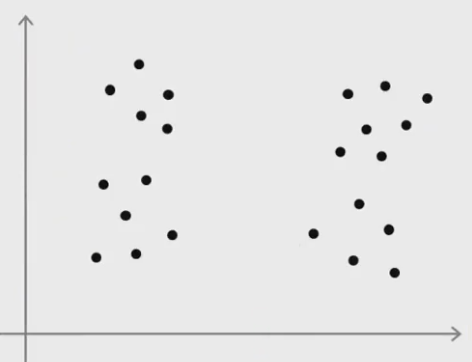
\includegraphics[scale=0.5]{sections/cs229/w10/amb.png}
	\end{center}

	\item The \textbf{elbow method} is to run $K$-means many times and vary the number of clusters.
	\begin{center}
		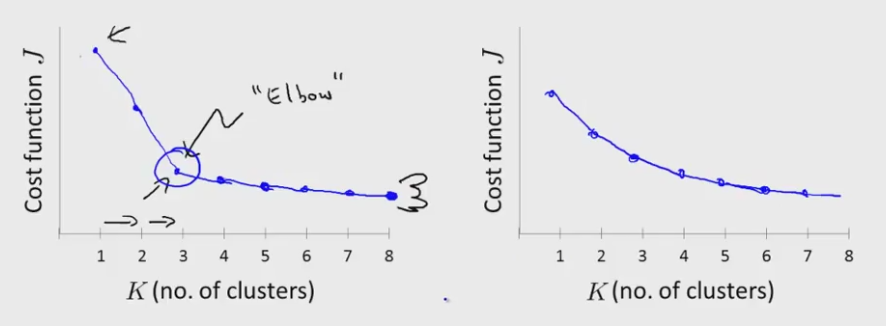
\includegraphics[scale=0.5]{sections/cs229/w10/elbow.png}
	\end{center}

	\item The method looks at the plot, and takes the ``elbow'' as the correct value
	\item The elbow method isn't typically used, because the curve can be just as ambiguous
	\item ``It's worth a shot, but don't have high expectations''
	\item Sometimes, you're running K-means to get clusters to ue for some later/downstream purpose. Evaluate K-means based on a metric for how well it performs for that later purpose
	\item 

\end{itemize}

	\subsection{Dimensionality Reduction}
	\subsubsection{Motivation I: Data Compression}
\begin{itemize}[--]
	\item Lets say we are given a data set, where 2 features are redundant (inches and cm), and we want to reduce the set to only account for 1 copy of this feature
	\item We can think of this reduction, as specifing the distance along the line that these dimensions chart

	\begin{center}
		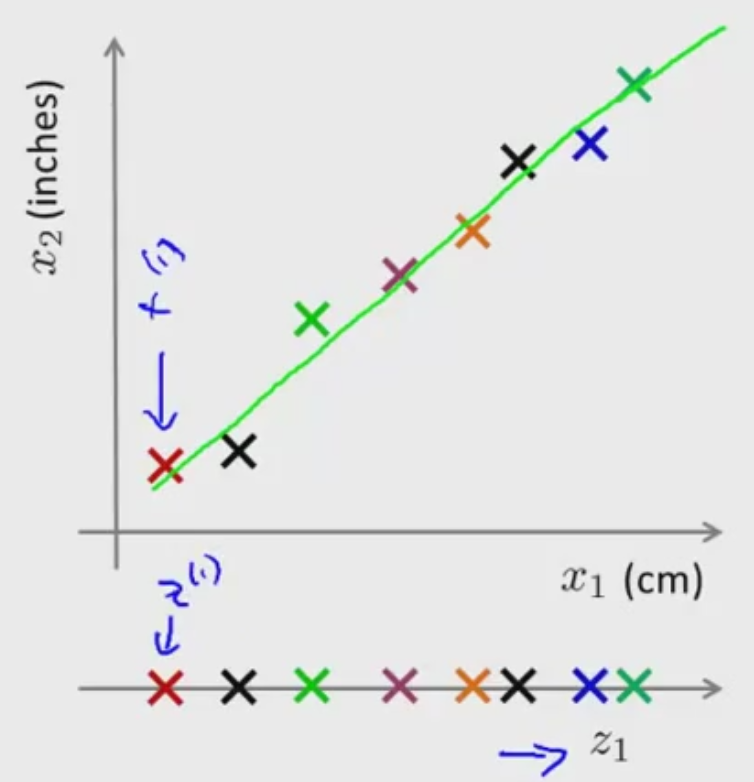
\includegraphics[scale=0.5]{sections/cs229/w11/2d_1d.png}
	\end{center}

	\item Here $z_1$ represents both $x_1$ and $x_2$
	\item This compression can happen from $m$-dimension to $n$-dimension ($m> n$), and is not limited to just one case
\end{itemize}

\subsubsection{Motivation II: Visualization}
\begin{itemize}[--]
	\item For a lot of problems, we want some way to visualize and understand the data 
	\item For example given $x^{(i)}\in\mathbb{R}^{50}$, using dimensionality reduction, we come up with a different feature representation $Z^{(i)}\in\mathbb{R}^2$ where these are some measure of the rest of the dimensions. Now we can chart this in on a plane.
\end{itemize}

\subsubsection{Principal Component Analysis Problem Formulation}
\begin{itemize}[--]
	\item PCA finds a lower dimensional surface on which to project the data, which minizes the projection error (distance from point to surface)
	\begin{center}
		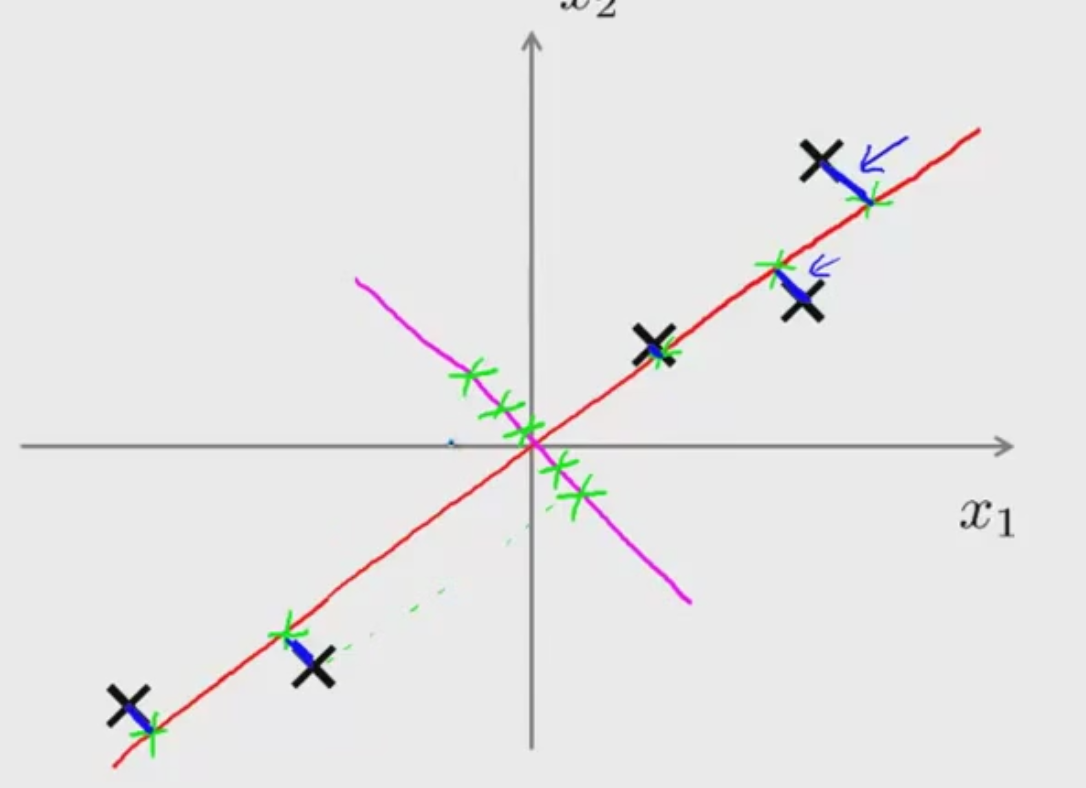
\includegraphics[scale=0.5]{sections/cs229/w11/bad.png}
	\end{center}

	\item There are bad choices (purple line) which have a very large error, and are not a good idea to reduce to, which is why we want to keep the error near zero
	\item \textbf{PCA}: Reduce from $n$-dimension to $k$-dimension: Find $k$ vectors $u^{(1)},\ldots,u^{(k)}$ onto which to project the data, so as to minimze the projection error
\end{itemize}

\subsubsection{Principal Component Analysis Algorithm}
\begin{itemize}[--]
	\item Data preprocessing
	\begin{itemize}[--]
		\item Training set: $x^{(1)},\ldots, x^{(m)}$
		\item Preprocessing (feature scaling/mean normalization);
			$$\mu_j = \frac{1}{m}\sum_{i=1}^{m}x_j^{(i)}$$
		\item Replace $x_j^{(i)}$ with $x_j - \mu_j$
		\item If different features on different scales (eg., $x_1=$size of house, $x_2=$ number of bedrooms), scale features to have comparable range of values
	\end{itemize}

	\item Reduce data from $n$-dimensions to $k$-dimensions
	\item Compute ``Covariance matrix'':
		$$\sigma = \frac{1}{m}\sum_{i=1}^{n} (x^{(i)})(x^{(i)})^T$$
	\item Compute eigenvectos of matrix $\sigma$: $[U, S, V] = svd(Sigma);$
	\item The $U$ matrix will have columns of the principal components $[u^{(i)}]$, since $U\in\mathbb{R}^{n\times n}$ we only need to take the first $k$ columns to reduce
		$$x\in\mathbb{R}^n\to z\in\mathbb{R}^k$$
		$$z= [\vec{u^{(1)}}, \ldots, \vec{u^{(k)}}]^{T} x $$
\end{itemize}

\subsubsection{Choosing the Number of Principal Components}
\begin{itemize}[--]
	\item Average squared projection error: $\frac{1}{m}\sum_{i=1}^{m} ||x^{(i)}- x_{approx}^{(i)} ||^2$
	\item Total variation in the data: $\frac{1}{m}\sum_{i=1}^{m}||x^{(i)}||^2$
	\item Typicall, choose $k$ to be the smallest value so that:
		$\frac{\text{Average squared proj error}}{\text{Total variation in data}}\leq 0.01$
	\item ``99\% of variance is retained''
	\item Algorithm:
	\begin{itemize}[--]
		\item Try PCA with $k=1:n$
		\item Compute $U_{reduce}, z^{(1)}, \ldots, z^{(m)}, x^{(1)}_{approx},\ldots, x^{(m)}_{approx}$
		\item Check if: $\leq 0.01$
	\end{itemize}

	\item When computing $[U, S, V]$, where $S$ is the diagonal matrix of eigenvalues
	\item For a given k:
		$$1-\frac{\sum_{i=1}^{k} S_{ii}}{\sum_{i=1}{n} S_{ii}}\leq 0.01$$
	\item This will give us the variability fraction like above
\end{itemize}

\subsubsection{Reconstrction from Compressed Representation}
\begin{center}
	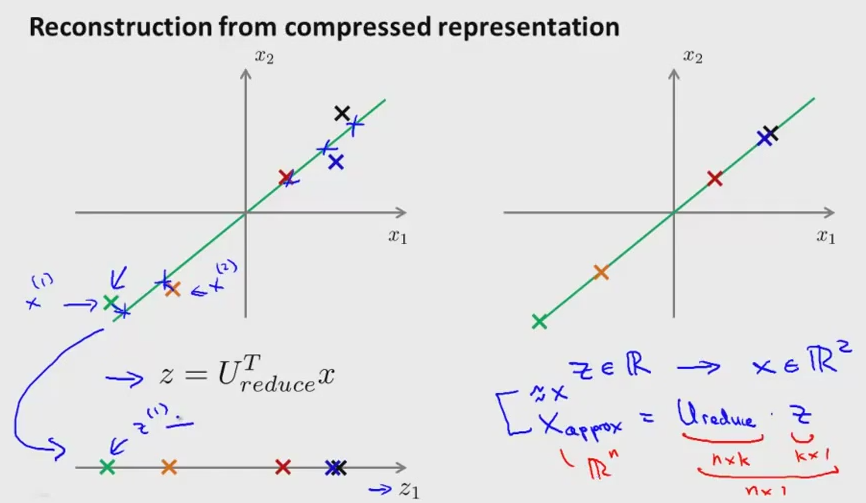
\includegraphics[scale=0.5]{sections/cs229/w11/reduce.png}
\end{center}
 
\subsubsection{Advice for Applying PCA}
\begin{itemize}[--]
	\item Suppose we have $(x^{(m)}, y^{(m)})$, $x^{(i)}\in\mathbb{R}^{10000}$ like in computer vision algorithms, running a learning algorithm will be very slow
	\item First extract inputs:
	\begin{itemize}[--]
		\item Unlabeled dataset: $x^{(1)},\ldots, x^{(m)}\in\mathbb{R}^{10000}$
		\item We convert via PCA into: $z^{(1)},\ldots, z^{(m)}\in\mathbb{R}^{1000}$
	\end{itemize}
	\item Now we have: $(z^{(1)}, y^{(1)})$, because our training examples are now represented with a lower dimension input
	\item Then we will learn our hypothesis: $h(z)$
	\item You should only reduce the training set, not the cv or test sets
	\item Bad use of PCA: To prevent overfitting:
	\begin{itemize}[--]
		\item Use $z^{(i)}$ instead of $x^{(i)}$ to reduce the number of features to $k < n$
		\item Thus, fewer features, less likely to overfit
		\item This might work OK, but isn't a good way to address overfitting. User regularization instead.
	\end{itemize}

	\item Consider, doing the whole thing without using PCA
	\item Before implementing PCA, first try running whatever you want to do with the original/raw data $x^{(i)}$. Only if that doesn't do what you want, then implement PCA and consider using $z^{(i)}$.

\end{itemize}


	\subsection{Anomaly Detection}
	\subsubsection{Problem Motivation}
\begin{itemize}[--]
	\item Imagine you're an aircraft engine manufacturing, and you measure multiple features $\{x^{(1)},\ldots ,x^{(m)} \}$ off your engines
	\item Lets say given a new engine $x_{test}$, is this aircraft engine anomalous in any way. Should it undergo further testing?
	\item If $p(x_{test}) < \epsilon\to$ flag anomaly
	\item Else $p(x_{test}) \geq\epsilon$ okay
	\item Applications:
	\begin{itemize}[--]
		\item Fraud detection
		\begin{itemize}[--]
			\item $x^{(i)}$ features of user $i$'s activities
			\item Model $p(x)$ from data
			\item Identify unusual users by checking which have $p(x) < \epsilon$
		\end{itemize}

		\item Manufacturing 
		\item Monitoring computers in a ata center
	\end{itemize}
\end{itemize}

\subsubsection{Gaussian Distribution}
\begin{itemize}[--]
	\item Say $x\in\mathbb{R}$. If $x$ is a distributed Gaussian with mean $\mu$, variance $\sigma^2$.
		$$x~\mathcal{N}(\mu, \sigma^2$$
	\item It will look like a bell shaped curve, with peak at $\mu$:
	\begin{center}
		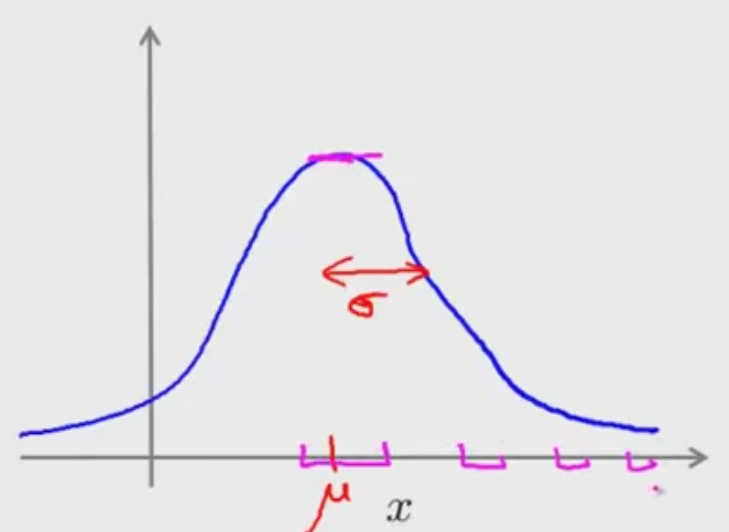
\includegraphics[scale=0.5]{sections/cs229/w12/gaus.png}
	\end{center}
	$$p(x;\mu, \sigma^2)=\frac{1}{\sqrt{2\pi}\sigma} \text{exp}(-\frac{(x-\mu)^2}{2\sigma^2})$$

	\item 
\end{itemize}

\subsubsection{Algorithm}
\begin{itemize}[--]
	\item Density estimation
	\begin{itemize}[--]
		\item Training set $\{ x^{(m)}\}\in\mathbb{R}^n$
			$$p(x)=p(x_1; \mu_1, \sigma_1^2 ) \ldots p(x_n; \mu_n, \sigma_n^2)$$
		\item This corresponds to an independnce assumption (not necessary to use this algorithm)
	\end{itemize}
	\item Algorithm:
	\begin{itemize}[--]
		\item Choose features $x_i$ that you think might be indicative of anomalous examples
		\item Fit parameters $\mu_1, \ldots, \mu_n, \sigma_1^2, \ldots, \sigma_n^2$
			$$\mu_j = \frac{1}{m}\sum_{i=1}^m x_j^{(i)}$$
			$$\sigma^{2}_j = \frac{1}{m}\sum_{i=1}^m (x_j^{(i)} - \mu_j )^2$$
		\item Given new example $x$, compute $p(x)$:
			$$p(x)=\prod_{j=1}^n p(x_j ; \mu_j, \sigma_j^2 )$$
		\item Anomaly if $p(x)< \epsilon$
	\end{itemize}
\end{itemize}

\subsubsection{Developing and Evaluating an Anomaly Detection System}
\begin{itemize}[--]
	\item When developing a learning algorithm (choosing features, etc.), making decisions is much easier if we have a way of evaluating our learning algorithm
	\item Assume we have some labeled data, of anomalous and non-anomalous examples ($y=0$ if normal, $y=1$ if anomalous).
	\item Training set: $x^{(1)},\ldots, x^{(m)}$ (assume normal examples/not anomalous)
	\item Cross validation set: $\{ (x_{cv}^{(m_{cv})}, y_{cv}^{(m_{cv})}\}$
	\item Test set: $\{ x_{test}^{(m_{test})}, y_{test}^{(m_{test})}\}$
	\item Given the aircraft example: 10000 good (normal) engines, 20 flawed engines (anomalous)
	\begin{itemize}[--]
		\item Training set: 6000 good engines ($y=0$)
		\item CV: 2000 good engines, 10 anomalous ($y=1$)
		\item Tset: 2000 good, 10 anomalous
	\end{itemize}

	\item Algorithnm evaluation:
	\begin{itemize}[--]
		\item Fit model $p(x)$ on training set $\{ x^{(m)}\}$
		\item On a cross validation/test example $x$, predict:
			$$y=\begin{cases}
				1 & p(x)< \epsilon \\
				0 & p(x) \geq\epsilon
			\end{cases}$$
		\item Possible evaluation metrics:
		\begin{itemize}[--]
			\item True positives, false positive, false negative, true negative
			\item Precision/Recall
			\item $F_1$ score
		\end{itemize}
		\item Can also use cross validation set to choose parameter $\epsilon$
	\end{itemize}
\end{itemize}

\subsubsection{Anomaly Detection vs. Supervised Learning}
\begin{itemize}[--]
	\item Anomaly Detection
	\begin{itemize}[--]
		\item Very small number of positive examples ($y=1$). (0-20 is common).
		\item Large number of negatives ($y=0$) examples
		\item Many differet ``types'' of anomalies. Hard for any algorithm to learn from positive examples what the anomalies look like; future anomalies may look nothing like any of the anomalous examples we've seen so far
	\end{itemize}

	\item Supervised Learning:
	\begin{itemize}[--]
		\item Large number of positive and negative examples
		\item Enough positive examples for algorithm to get a sense of what positive examples are like, future positive examples likely tob e similar to ones in training set
	\end{itemize}

	\item In anomaly detection, we typically have very small postivie examples, so there's not enough to learn about them
\end{itemize}

\subsubsection{Choosing What Features to Use}
\begin{itemize}[--]
	\item When plotting the probabilities from the anomaly detection we hope to get a gaussian distribution:
	\begin{center}
		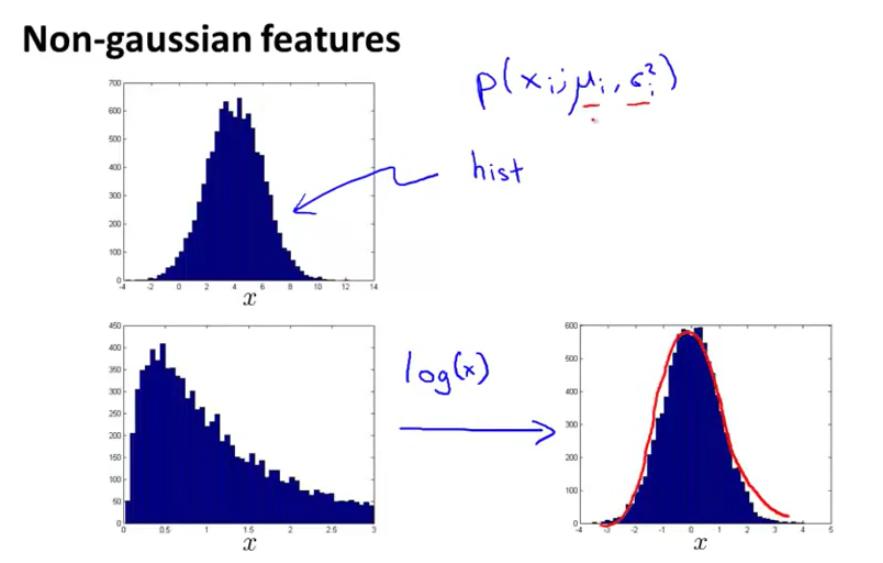
\includegraphics[scale=0.5]{sections/cs229/w12/gausfeat.png}
	\end{center}
	\item However, sometimes we get a skewed distribution, and it's best to attempt to transform (eg. $\log{x_i + c}\to x_i$) this data into a guassian distribution.
	\item Error analysis for anomaly detection
	\begin{itemize}[--]
	 	\item Want $p(x)$ large for normal examples $x$, and small for anomalous examples
	 	\item Most common problem: $p(x)$ is comparable (say, both large) for normal and anomalous examples
	 	\item One way to help pull out the anomaly, is to come up with another feature that makes it easier to distinguish anomalies 
	 \end{itemize}
	 \item Choose features that might take on unusally large or small values in the vent of an anomaly (eg. network traffic, CPU load)
\end{itemize}

\subsubsection{Multivariate Gaussian Distribution}
\begin{itemize}[--]
	\item Lets say we have unlabelled data:
	\begin{center}[--]
		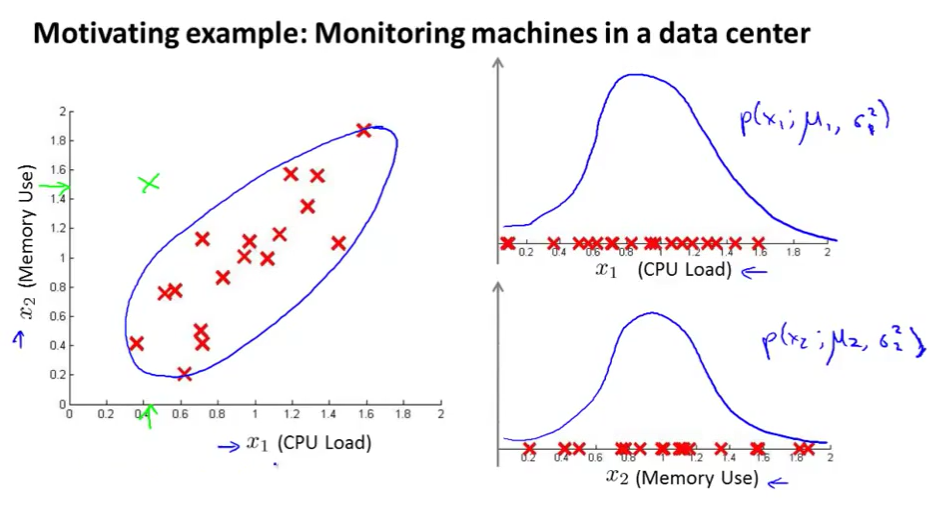
\includegraphics[scale=0.5]{sections/cs229/w12/multi.png}
	\end{center}
	\item Where we have an anomaly (green)
	\item This anomaly, doesn't appear to be an outlier in either 1D plot
	\item This keeps a 	`circular' regions of probability
	\item $x\in\mathbb{R}^{n}$. Don't model $p(x_1),\ldots$ separately. Model $p(x)$ all in one go.
	\item Parameters: $\mu\in\mathbb{R}^n$, $\sigma\in\mathbb{R}^{n\times n}$ (covariance matrix)
		$$p(x;\mu, \sigma)=\frac{1}{(2u\pi)^{n/2} |\sigma |^{0.5}} \text{exp} (-0.5 (x-\mu)^T \sigma^{-1} (x-\mu))$$
	\begin{center}[--]
		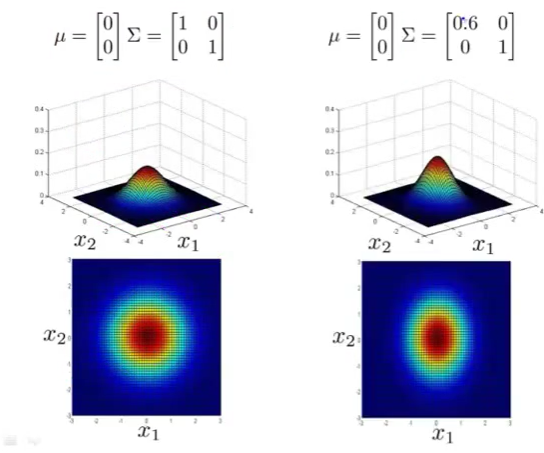
\includegraphics[scale=0.5]{sections/cs229/w12/ex.png}
	\end{center}
	\item As you decrease $\sigma$ you get a smaller steeper curve, in the direction of the col/row you varied
	\item $\mu$ similarly models the point where the curve is centered
	\item You can also model correlactions with the off-diagonal entries
	\begin{center}[--]
		% 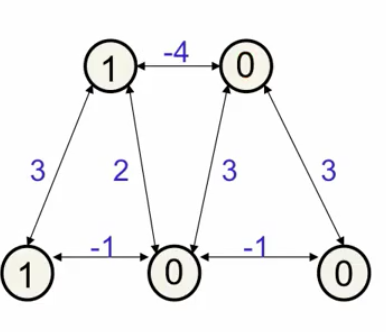
\includegraphics[scale=0.5]{sections/cs229/w12/off.png} TODO: get
	\end{center}
\end{itemize}

\subsubsection{Anomaly Detection using the Multivariate Gaussian Distribution}
\begin{itemize}[--]
	\item Given a training set: $\{ x^{(m)}\}\in\mathbb{R}^n$
		$$\mu = \frac{1}{m}\sum_{i=1}^{m} x^{(i)}$$
		$$\sigma = \frac{1}{m}\sum_{i=1}^{m} (x^{(i)}-\mu ) (x^{(i)}-\mu ) ^T$$
	\item Fit model $p(x)$ by setting these previous parameters	
	\item Given a new example $x$, compute:
		$p(x;\mu, \sigma^2)$
		Flag an anomaly if $p(x)<\epsilon$
	\item The original product model of Gaussian, corresponds to multivariate Gaussian where the distribution is constrained so that the contours are axis aligned
	\item Namely, $\sigma$ has 0's on the off-diagonal entries
	\item When would you use each?
	\item \textbf{Original Model}
	\begin{itemize}[--]
		\item Manually create features to capture anomalies where $x_1, x_2$ takes unusual combinations of values (eg. $x_3=x_1/x_2$)
		\item If you're willing to spend the time creating these features, this model will work fine
		\item Computationally cheaper (alternatively, scalles better to large $n$)
		\item OK even if $m$ (training set size) is small
	\end{itemize}

	\item \textbf{Multivariate Gaussian}
	\begin{itemize}[--]
		\item Automatically captures correlations between features
		\item Computationally more expensive
		\item Must have $m>n$, or else $\sigma$ is non-inverible
		\item $\sigma$ may be non-invertible if there are redundant features ($x_1=x_2, x_3 = x_4 + x_5$), linearly dependent.
	\end{itemize}
\end{itemize}

	\subsection{Recommender Systems}
	\subsubsection{Problem Formulation}
\begin{itemize}[--]
	\item Example: predicting movie ratings. Want to recommend movies that people will enjoy.
	\item User rates movies using zero-to-five stars \\
	\begin{center}\begin{tabular}{c | c c c c}
		\textbf{Movie} & \textbf{Alice (1)} & \textbf{Bob (2)} & \textbf{Carol (3)} & \textbf{Dave (4)} \\ \hline
		Love at last & 5 & 5 & 0 & 0 \\
		Romance forever & 5 & ? & ? & 0 \\
		Cute puppies of love & ? & 4 & 0 & ? \\
		Nonstop car chases & 0 & 0 & 5 & 4 \\
		Swords vs. karate & 0 & 0 &  5 & ?
	\end{tabular}\end{center}
	\item Notation
	\begin{itemize}[--]
		\item $n_u=$ no. users
		\item $n_m=$ no. movies
		\item $r(i,j)=$ 1 if user $j$ has rated movie $i$
		\item $y^{(i,j)}=$ rating given by user $j$ to movie $i$ (defined only if $r(i,j)=1$)
	\end{itemize}
	\item We want to predict what the `?' will be in our table, namely, how much they will like the movie
	\item In our data, we can see Alice and Bob like romance movies, and not so much action movies. We want to be able to learn from this and recommend movies intelligently based on this sort of information
\end{itemize}

\subsubsection{Content Based Recommendations}
\begin{itemize}[--]
	\item Say we define features based on different recommendation categories: \\
	\begin{center}\begin{tabular}{c | c c c c | c c}
		\textbf{Movie} & \textbf{Alice (1)} & \textbf{Bob (2)} & \textbf{Carol (3)} & \textbf{Dave (4)} & $x_1$ (romance) & $x_2$ (action\\ \hline
		Love at last & 5 & 5 & 0 & 0 & 0.9 & 0\\
		Romance forever & 5 & ? & ? & 0 & 1 & 0.01\\
		Cute puppies of love & ? & 4 & 0 & ? & 0.99 & 0\\
		Nonstop car chases & 0 & 0 & 5 & 4 & 0.1 & 1\\
		Swords vs. karate & 0 & 0 &  5 & ? & 0 & 0.9
	\end{tabular}\end{center}
	\item With this dat we have: $n_u=4, n_m=5$. We also include our intercept term: $x_0=1$
		$$x^{(1)}=\begin{bmatrix}
			1\\
			0.9\\
			0
		\end{bmatrix}$$
	\item For each user $j$, learn a paramter $\theta^{(j)}\in\mathbb{R}^3$. Predict user $j$ as rating movei $i$ with $(\theta^{(j)})^T x^{(i)}$ stars.
	\item Suppose we want to want to guess what Alice will think of ``Cute puppies of love'':
		$$x^{(3)}=\begin{bmatrix}
			1 \\ 0.99 \\ 0
		\end{bmatrix}, \theta^{(1)}=\begin{bmatrix}
			0 \\ 5 \\ 0
		\end{bmatrix}, (\theta^{(1)})^T x^{(3)} = 4.95$$
	\item We will discuss how we got $\theta$ later.
	\item We would predict that Alice would enjoy the movie 
	\item Problem formulation:
	\begin{itemize}[--]
		\item $r(i, j)=1$ if user $j$ has rated movie $i$ (0 otherwise)
		\item $y^{(i,j)}=$ rating by user $j$ on movie $i$ (if defined)
		\item $\theta^{(j)}=$ parameter vector for user $j$
		\item $x^{(i)}=$ feature vector for movei $i$
		\item For user $j$, movie $i$, predicted rating: $(\theta^{(j)})^T x^{(i)}$
		\item $m^{(j)}=$ no. of movies rated by user $j$
		\item To learn $\theta^{(j)}$ (paramter for user $j$):
			$$\min_{\theta^{(j)}}\frac{1}{2m^{(j)}}\sum_{i:r(i,j)=1} ((\theta^{(j)})^T x^{(i)} - y^{(i,j)})^2 + \frac{\lambda}{2m^{(j)}}\sum_{k=1}^n (\theta_k^{(j)})^2$$
		\item To learn $\theta^{(1)},\ldots, \theta^{(n_u)}$:
			$$\min_{\theta^{(1)},\ldots, \theta^{(n_u)}}\frac{1}{2m^{(j)}}\sum_{j=1}^{n_u}\sum_{i:r(i,j)=1} ((\theta^{(j)})^T x^{(i)} - y^{(i,j)})^2 + \frac{\lambda}{2m^{(j)}}\sum_{j=1}^{n_u}\sum_{k=1}^n (\theta_k^{(j)})^2$$
		\item Gradient descent update:
			$$\theta_k^{(j)}:=\theta_k^{(j)} - \alpha\sum_{i:r(i,j)=1}((\theta^{(j)})^T x^{(i)} - y^{(i,j)})x_k^{(i)} \text{ for } k =0$$
			$$\theta_k^{(j)}:=\theta_k^{(j)} - \alpha ( \sum_{i:r(i,j)=1}((\theta^{(j)})^T x^{(i)} - y^{(i,j)})x_k^{(i)} +\lambda\theta_k^{(j)} ) \text{ for } k \neq 0$$
			
	\end{itemize}
	\item Since $m^{(j)}$ is a constant, you may exclude it to simplify the math
\end{itemize}

\subsubsection{Collaborative Filtering}
\begin{itemize}[--]
	\item One of the movies has a feature vector $x^{(1)}$, we can infer from the opinions (the $\theta$) of the individuals the type of movie we are looking at
	\item Given $\theta^{(1)},\ldots, \theta^{(n_u)}$, to learn $x^{(i)}$:
		$$\min_{x^{(i)}}\frac{1}{2}\sum_{j:r(i,j)=1}((\theta^{(j)})^T x^{(i)} - y^{(i,j)})^2 + \frac{\lambda}{2}\sum_{k=1}^n (x_k^{(i)})^2$$
	\item Given $\theta^{(1)},\ldots,\theta^{(n_u)}$ to learn $x^{(1)},\ldots , x^{(n_m)}$:
		$$\min_{x^{(i)}}\frac{1}{2}\sum_{i=1}^{n_m}\sum_{j:r(i,j)=1}((\theta^{(j)})^T x^{(i)} - y^{(i,j)})^2 + \frac{\lambda}{2}\sum_{i=1}^{n_m}\sum_{k=1}^n (x_k^{(i)})^2$$
	\item Given $x^{(n_m)}$ (and omvie ratings), can estimate $\theta^{(n_u)}$
	\item Given $\theta^{(n_u)}$, can estimate $x^{(n_m)}$
	\item Which do we want to do first?
	\item Guess $\theta\to x\to\theta\to x\to\ldots$
	\item This will cause your features to converge via \textbf{collaborative filtering}
\end{itemize}

\subsubsection{Collaborative Filtering Algorithm}
\begin{itemize}[--]
	\item Collaborative filtering optimization objective:
		$$J(x^{(1)},\ldots,x^{(n_m)},\theta^{(1)},\ldots,\theta^{(n_u)}=\frac{1}{2}\sum_{(i,j):r(i,j)=1}((\theta^{(j)})^T x^{(i)} - y^{(i,j)})^2 + \frac{\lambda}{2}\sum_{i=1}^{n_m}\sum_{k=1}^{n} (x_k^{(i)})^2 + \frac{\lambda}{2}\sum_{j=1}^{n_u}\sum_{k=1}^{n} (\theta_k^{(j)})^2$$

		$$\min_{x^{(1)},\ldots, x^{(n_m)}, \theta^{(1)},\ldots,x^{(n_u)}} J(\ldots)$$

	\item Algorithm:
	\begin{itemize}[--]
		\item Initialize $x^{(n_m)}, \theta^{(n_u)}$ to small random values
		\item Minimize $J(\ldots)$ using gradient descent (or an advanced optimization algorithm) eg. for every $j=1,\ldots,n_u, i=1,\ldots n_m$:
			$$x_k^{(i)}:= x_k^{(i)} - \alpha \left(
				\sum_{j:r(i,j)=1} ((\theta^{(j)})^T x^{(i)} - y^{(i,j)})\theta_k^{(j)} +\lambda x_k^{(i)}
			\right)$$
			$$\theta_k^{(j)}:=\theta_k^{(j)} - \alpha \left(
				\sum_{i:r(i,j)=1} ((\theta^{(j)})^T x^{(i)} - y^{(i,j)})x_k^{(i)} +\lambda \theta_k^{(j)}
			\right)$$
		\item For a user with parameters $\theta$ and a movie with (learned) features $x$, predict a star rating of $\theta^T x$
	\end{itemize}
\end{itemize}

\subsubsection{Vectorization - Low Rank Matrix Factorization}
\begin{itemize}[--]
	\item Lets group the movie data into a matrix:
		$$Y=\begin{bmatrix}
			5 & 5 & 0 & 0 \\
			5 & ? & ? & 0 \\
			? & 4 & 0 & ? \\
			0 & 0 & 5 & 4 \\
			0 & 0 & 5 & 0
		\end{bmatrix}$$
	\item This is what we were previously writing sa $y^{(i,j)}$
	\item Predicted ratings:
		$$\begin{bmatrix}
			(\theta^{(1)})^Tx^{(1)} & (\theta^{(2)})^Tx^{(1)} & \ldots & (\theta^{(n_u)})^Tx^{(1)} \\
			(\theta^{(1)})^Tx^{(2)} & (\theta^{(2)})^Tx^{(2)} & \ldots & (\theta^{(n_u)})^Tx^{(2)} \\
			\vdots & \vdots & \ddots & \vdots \\
			(\theta^{(1)})^Tx^{(n_m)} & (\theta^{(2)})^Tx^{(n_m)} & \ldots & (\theta^{(n_u)})^Tx^{(n_m)}
		\end{bmatrix}$$\
	\item We can denote vectorize this via:
		$$X=\begin{bmatrix}
			\rule[.5ex]{.5em}{0.4pt} & (x^{(1)})^T & \rule[.5ex]{.5em}{0.4pt} \\
			\rule[.5ex]{.5em}{0.4pt} & (x^{(2)})^T & \rule[.5ex]{.5em}{0.4pt} \\
			& \vdots \\
			\rule[.5ex]{.5em}{0.4pt} & (x^{(n_m)})^T & \rule[.5ex]{.5em}{0.4pt} \\
		\end{bmatrix}, \Theta=\begin{bmatrix}
			\rule[.5ex]{.5em}{0.4pt} & (\theta^{(1)})^T & \rule[.5ex]{.5em}{0.4pt} \\
			\rule[.5ex]{.5em}{0.4pt} & (\theta^{(2)})^T & \rule[.5ex]{.5em}{0.4pt} \\
			& \vdots \\
			\rule[.5ex]{.5em}{0.4pt} & (\theta^{(n_u)})^T & \rule[.5ex]{.5em}{0.4pt} \\
		\end{bmatrix}$$
		$$X\Theta^T$$
	\item This algorithm is also called \textbf{low rank matrix factorization}
	\item This matrix has a mathematical property called \textbf{low rank matrix}
	\item Finding related movies:
	\begin{itemize}[--]
		\item For each product $i$, we learn a feature vector $x^{(i)}\in\mathbb{R}^n$
		\item Potential features: $x_1 = $ romance, $x_2 = $ action, $\ldots$
		\item It's hard to truely interpret for a human in practice
		\item How to find movies $j$ related to movie $i$?
		\item $||x^{(i)} - x^{(j)}||$ is small $\to$ movie $j$ and $i$ are ``similar'' 
	\end{itemize}
\end{itemize}

\subsubsection{Implementaiton Detail - Mean Normalization}
\begin{itemize}[--]
	\item Consider a user who has not rated any movies
	\item $n=2, \theta^{(5)}\in\mathbb{R}^2$, but he has no movies which are rated
	\item So only the regularization term afffects $\theta^{(5)}$, since the first term in the cost function is unknown
	\item This will result in: $\theta^{(5)}=\vec{0}$
	\item This assumption of ranking all movies with a 0, doesn't seem very likely
	\item For \textbf{mean normalization} we will compute the average rating as so:
		$$\mu=\begin{bmatrix}
			2.5 \\ 2.5 \\ 2 \\ 2.25 \\ 1.25
		\end{bmatrix}$$
	\item Then we perform: $Y:= Y - \mu$
	\item We will use these mean normalized movie ratings to learn $\theta^{(j)}, x^{(i)}$
	\item For user $j$, on movie $i$ predict:
		$$(\theta^{(j)})^Tx^{(i)} + \mu_i$$
	\item This will result in our new user to have average ratings as a guess
 \end{itemize}

	\subsection{Large Scale Machine Learning}
	\subsubsection{Learning with Large Datasets}
\begin{itemize}[--]
	\item We want to use larger datasets because it can significantly improve our models
	\item Learning with large datasets comes with its own problems, typically computational times
	\item For example: gradient descent's update term is $\O{m}$, for each update of $\theta_j$
	\item Why not randomly choose a subset of data to train on before investing effort into creating software for large datasets
	\item If you plot can already show that $J_{cv}\approx J_{train}$ then you're already set, so there's no need to scale
\end{itemize}

\subsubsection{Stochastic Gradient Descent}
\begin{itemize}[--]
	\item Linear regression with gradient descent:
	\begin{center}
		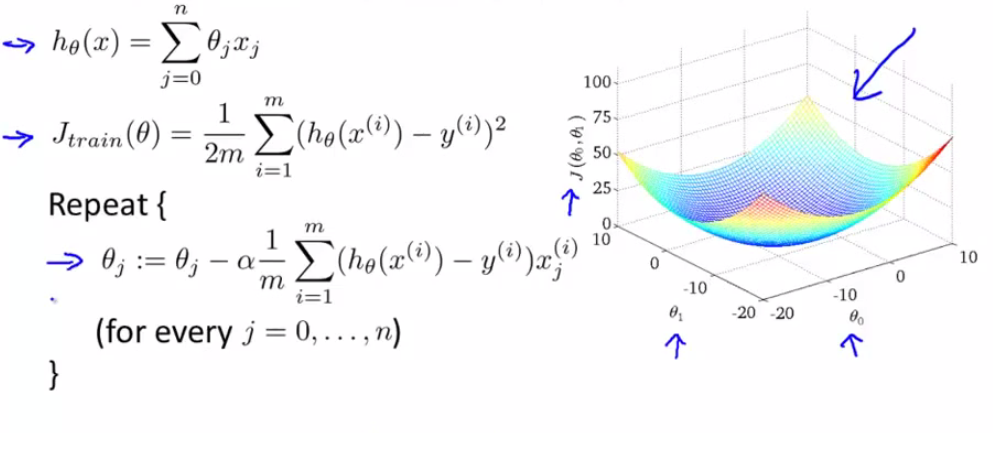
\includegraphics[scale=0.5]{sections/cs229/w14/grad_desc.png}
	\end{center}
	\item The ideas we will present are fully general, but we will use linear regression to exemplify
	\item The previous version of gradient descent we used is called \textbf{batch gradient descent}, because we're looking at a batch of examples
	\item We will redefine:
		$$cost(\theta, (x^{(i)}, y^{(i)})) = \frac{1}{2} (h(x^{i)}) - y^{(i)})^2$$
	\item We can now rewrite:
		$$J_{train}=\frac{1}{m}\sum_{i=1}^m cost(\theta, (x^{(i)}, y^{(i)}))$$
	\item Stochastic gradient descent:
	\begin{itemize}[--]
		\item Randomly suffle dataset
		\item Repeat\{ \\
			for i=1,$\ldots$,m\{ \\
				$\theta_j := \theta_j - \alpha (h(x^{(i)}) - y^{(i)})x_j^{(i)}$ for $j=0,\ldots,n$ \\
			\} \\
		\}
	\end{itemize}
	\item It's scanning through the training examples, and take a gradient descent step with the cost of just the first training example, repeating to fit a little towards each training example
	\item This outter loop allows multiple movements through the data set
	\item Batch gradient descent would make a reasonable move towards the center; however, stochastic will move more randomly as it conforms to each example
	\item It wanders around the global minimum, not necessarly finding it in the end; however, this shouldn't matter too much in most models in pratice
	\item How many times should we repeat the outer loop? 1-10x may be enough depending on the training set
\end{itemize}

\subsubsection{Mini-Batch Gradient Descent}
\begin{itemize}[--]
	\item Batch gradient descent: Use all $m$ examples in each iteration
	\item Stochastic gradient descent: USe 1 example in each iteration
	\item Mini-batch gradinet descent: Use $b$ examples in each iteration
	\item $b=$ mini-batch size (Typical range: [2, 100])
	\item This changes our update towards:
		$$\theta_j := \theta_j - \alpha\frac{1}{b}\sum_{k=i}^{i+b-1} (h(x^{(k)}) - y^{(k)} x_j^{(k)}$$
		$$i := i + b$$
	\item 
\end{itemize}

\subsubsection{Stochastic Gradient Descent Convergence}
\begin{itemize}[--]
	\item For batch gradient descent, we would plot $J_{train}$ as a function of the number of iterations, ensuring that it remained decreasing
	\item However with stochastic, you can't check the same cost function, because it uses the slow technique that it's designed to avoid
	\item Instead during learning, compute $cost(\theta, (x^{(i)}, y^{(i)}))$ before updating $\theta$ using $(x^{(i)}, y^{(i)})$
	\item Now every so many interations (say 1000) iterations, plot $cost$ averaged over the last 1000 examples processed by the algorithm
	\item These plots may be noisy
	\item As you increase the number of iterations you average, you may be able to achieve a smoother curve, but you get very little feedback
	\item Somtiems the cost won't decrease, but when increasing the iterations you may get more intution that is hidden by the noise
	\item If the curve diverges, use a smaller learning rate $\alpha$
	\item Learning rate $\alpha$ is typically held constant. It can slowly decrease over time if we want $\theta$ to converge
	\item This may not be worthwhile since you have to tune more paramteres
\end{itemize}

\subsubsection{Online Learning}
\begin{itemize}[--]
	\item If you have a continuous stream of data is use an online learning algorithm to use the prefences from the stream of data to optimize some of the decisions on the site
	\item Considering a shipping service webstie where user comes, specifies origin and destination, you offer to ship their package for some asking price, and users sometimes choose to use your shipping services ($y=1$), and sometimes not ($y=0$)
	\item Features $x$ capture properties of user, of origin/destination and asking price. We want to learn $p(y=1|x;\theta)$ to optimize price
	\item Repeat forever \{
	Get $(x,y)$ corresponding to user.
	Update $\theta$ using just the new example $(x,y)$:
		$\theta_j := \theta_j - \alpha (h(x) - y)x_j$ for $j=0,\ldots, n$
	\}
	\item We are discarding the notion of a fix training set, so no longer using ${(i)}$ notation
	\item This algorithm can adapt to changing user preferences
	\item Another example: Product search (learning to search)
	\begin{itemize}[--]
		\item User searches for ``android phone 1080p camera''
		\item Have 100 phones in store. Will return 10 results.
		\item $x=$ features of phone, how many words in user query match name of phne, how many words in query match description of phone, etc.
		\item $y=1$ if user clicks on link. $y=0$ otherwise
		\item Learn $p(y=1|x;\theta)$
		\item Learning the CTR (click-through-rate)
		\item Use to show user the 10 phones they're most likely to click on
	\end{itemize}
	\item Other examples: choosing special offers to show user; customized selection of news articles; product recommendations $\ldots$
\end{itemize}

\subsubsection{Map Reduce and Data Parallelism}
\begin{itemize}[--]
	\item We will split the training set into different subsets, and process each portion on a different computer
	\item After each machine as computed a temporary new $\theta_j$ and combine them 
		$$\theta_j := \theta_j - \alpha \frac{1}{m} (temp_j^{(1)}+\ldots+temp_j^{(\ldots)} \text{ for } j = 0,\ldots, n$$
	\item Many learning algorithms can be expressed as computing sums of functiosn over the training set
	\item You can also use this on multi-core machines
	\item Some linear algebra libraries already do multi-core computations
\end{itemize}

	\subsection{Application Example: Photo OCR}
	\subsubsection{Problem Descritpion and Pipeline}
\begin{itemize}[--]
	\item \textbf{Photo OCR}: photo optical character recognition
	\item How do we get computers to understand the text that appears in images
	\item Photo OCR pipeline
	\begin{itemize}[--]
		\item Text detection (bounding box)
		\item Character segmentation (segment each character within box)
		\item Character classification (on each segment)
	\end{itemize}
	\item These `pipelines' are common, where each component may be its own machine learning component (not necessary)
	\item This pipeline can be one of the most important design decision
\end{itemize}

\subsubsection{Sliding Windows}
\begin{itemize}[--]
	\item Supervised leanring for pedestrain detection:
	\begin{itemize}[--]
		\item $x=$ pixels in 82x36 image patches
		\item Positive examples ($y=1$), negative ($y=0$)
		\item Where positive examples are images containing a pedestrian
		\item Train a classifier to recognize pedestrians
	\end{itemize}
	\item To check if if a pedestrian in our image, we will take the same bounding box and slide it across the first row of this size on our image
	\item The amount of pixels you shift the image over in this slide is called the \textbf{step-size/stride}
	\item Now we scale this sliding box for different sized objects of interest
	\item We can apply this concept to detect boxes that contain some sort of character
	\item We can expand our guessed areas, and then draw bounding rectangles over areas that have reasonable resolutions for words
	\item We may also need to train a classifier to classify between letters that are split/partial, to find the individual characters in the words
\end{itemize}

\subsubsection{Getting Lots of Data and Artificial Data}
\begin{itemize}[--]
	\item For character recognition, we can make fake data by taking font from the internet and overlaying it on a random background iamge
	\item You can apply different distortions to get even more sophisticated examples
	\item Another way is by taking already obtained data, and introducing distortions
	\item For another example you can alter audio for speech recognition by overlaying backgrounds
	\item Distortion introduced should be representation of the type of noise/distortions in test set
	\item Usually does not help to add purely random/meaningless noise to your data
	\item Discussion on getting more data:
	\begin{itemize}[--]
		\item Make sure you have a low bias classifier before expending the effort (Plot learning curves). eg. keep increasing the number of features/number of hidden units in neural network until you have a low bias classifier
		\item  ``How much work would it be to get 10x as much data as we currently have?''
		\begin{itemize}[--]
			\item Artificial data synthesis
			\item Collect/label it yourself (no. of hours?)
			\item ``Crowd source'' (eg. amazon mechanical turk)
		\end{itemize}
	\end{itemize}
\end{itemize}

\subsubsection{Ceiling Analysis - What Part of the Pipeline to Work on Next}
\begin{itemize}[--]
	\item  What part of the pipeline should you spend the most time trying to improve?
	\item In order to make decisions on developing the system, it will be helpful to have a single real-number evaluation of the system
	\item Feed perfect inputs into each pipeline stage and see the total improvement via this metric
	\item The larger the jump, the more you should focuso on that segment of the pipeline
\end{itemize}



% \section{Introduction and Overview}
% \section{Supervised Learning: Regression}
% \section{Supervised Learning: Classification}
% \section{Kernel Methods}
% \section{Regularization and Model Selection}
% \section{Advice on using ML Algorithms}
% \section{Neural Networks}
% \section{Unsupervised Learning}
% \section{Gaussian Process}
% \section{Ensemble Methods}
% \section{Sequence Modeling}
% \section{Learning Theory}

\end{document}